\chapter{基于实时路况的调度系统设计}

本章首先介绍了基于区块链的出租车调度系统结构,然后介绍了传统A*算法的工作原理,并在此基础上结合实时路况,提出了一种改进后的A*算法,最后将改进后的A*算法与出租车调度系统融合,形成一个基于实时路况的出租车调度系统。
% 第三章的开头加一节,展现整个系统的结构,包括系统组成部分,各部分的相互关系和接口。

\section{基于区块链的调度系统结构分析}

\begin{figure}[ht]
  \centering
  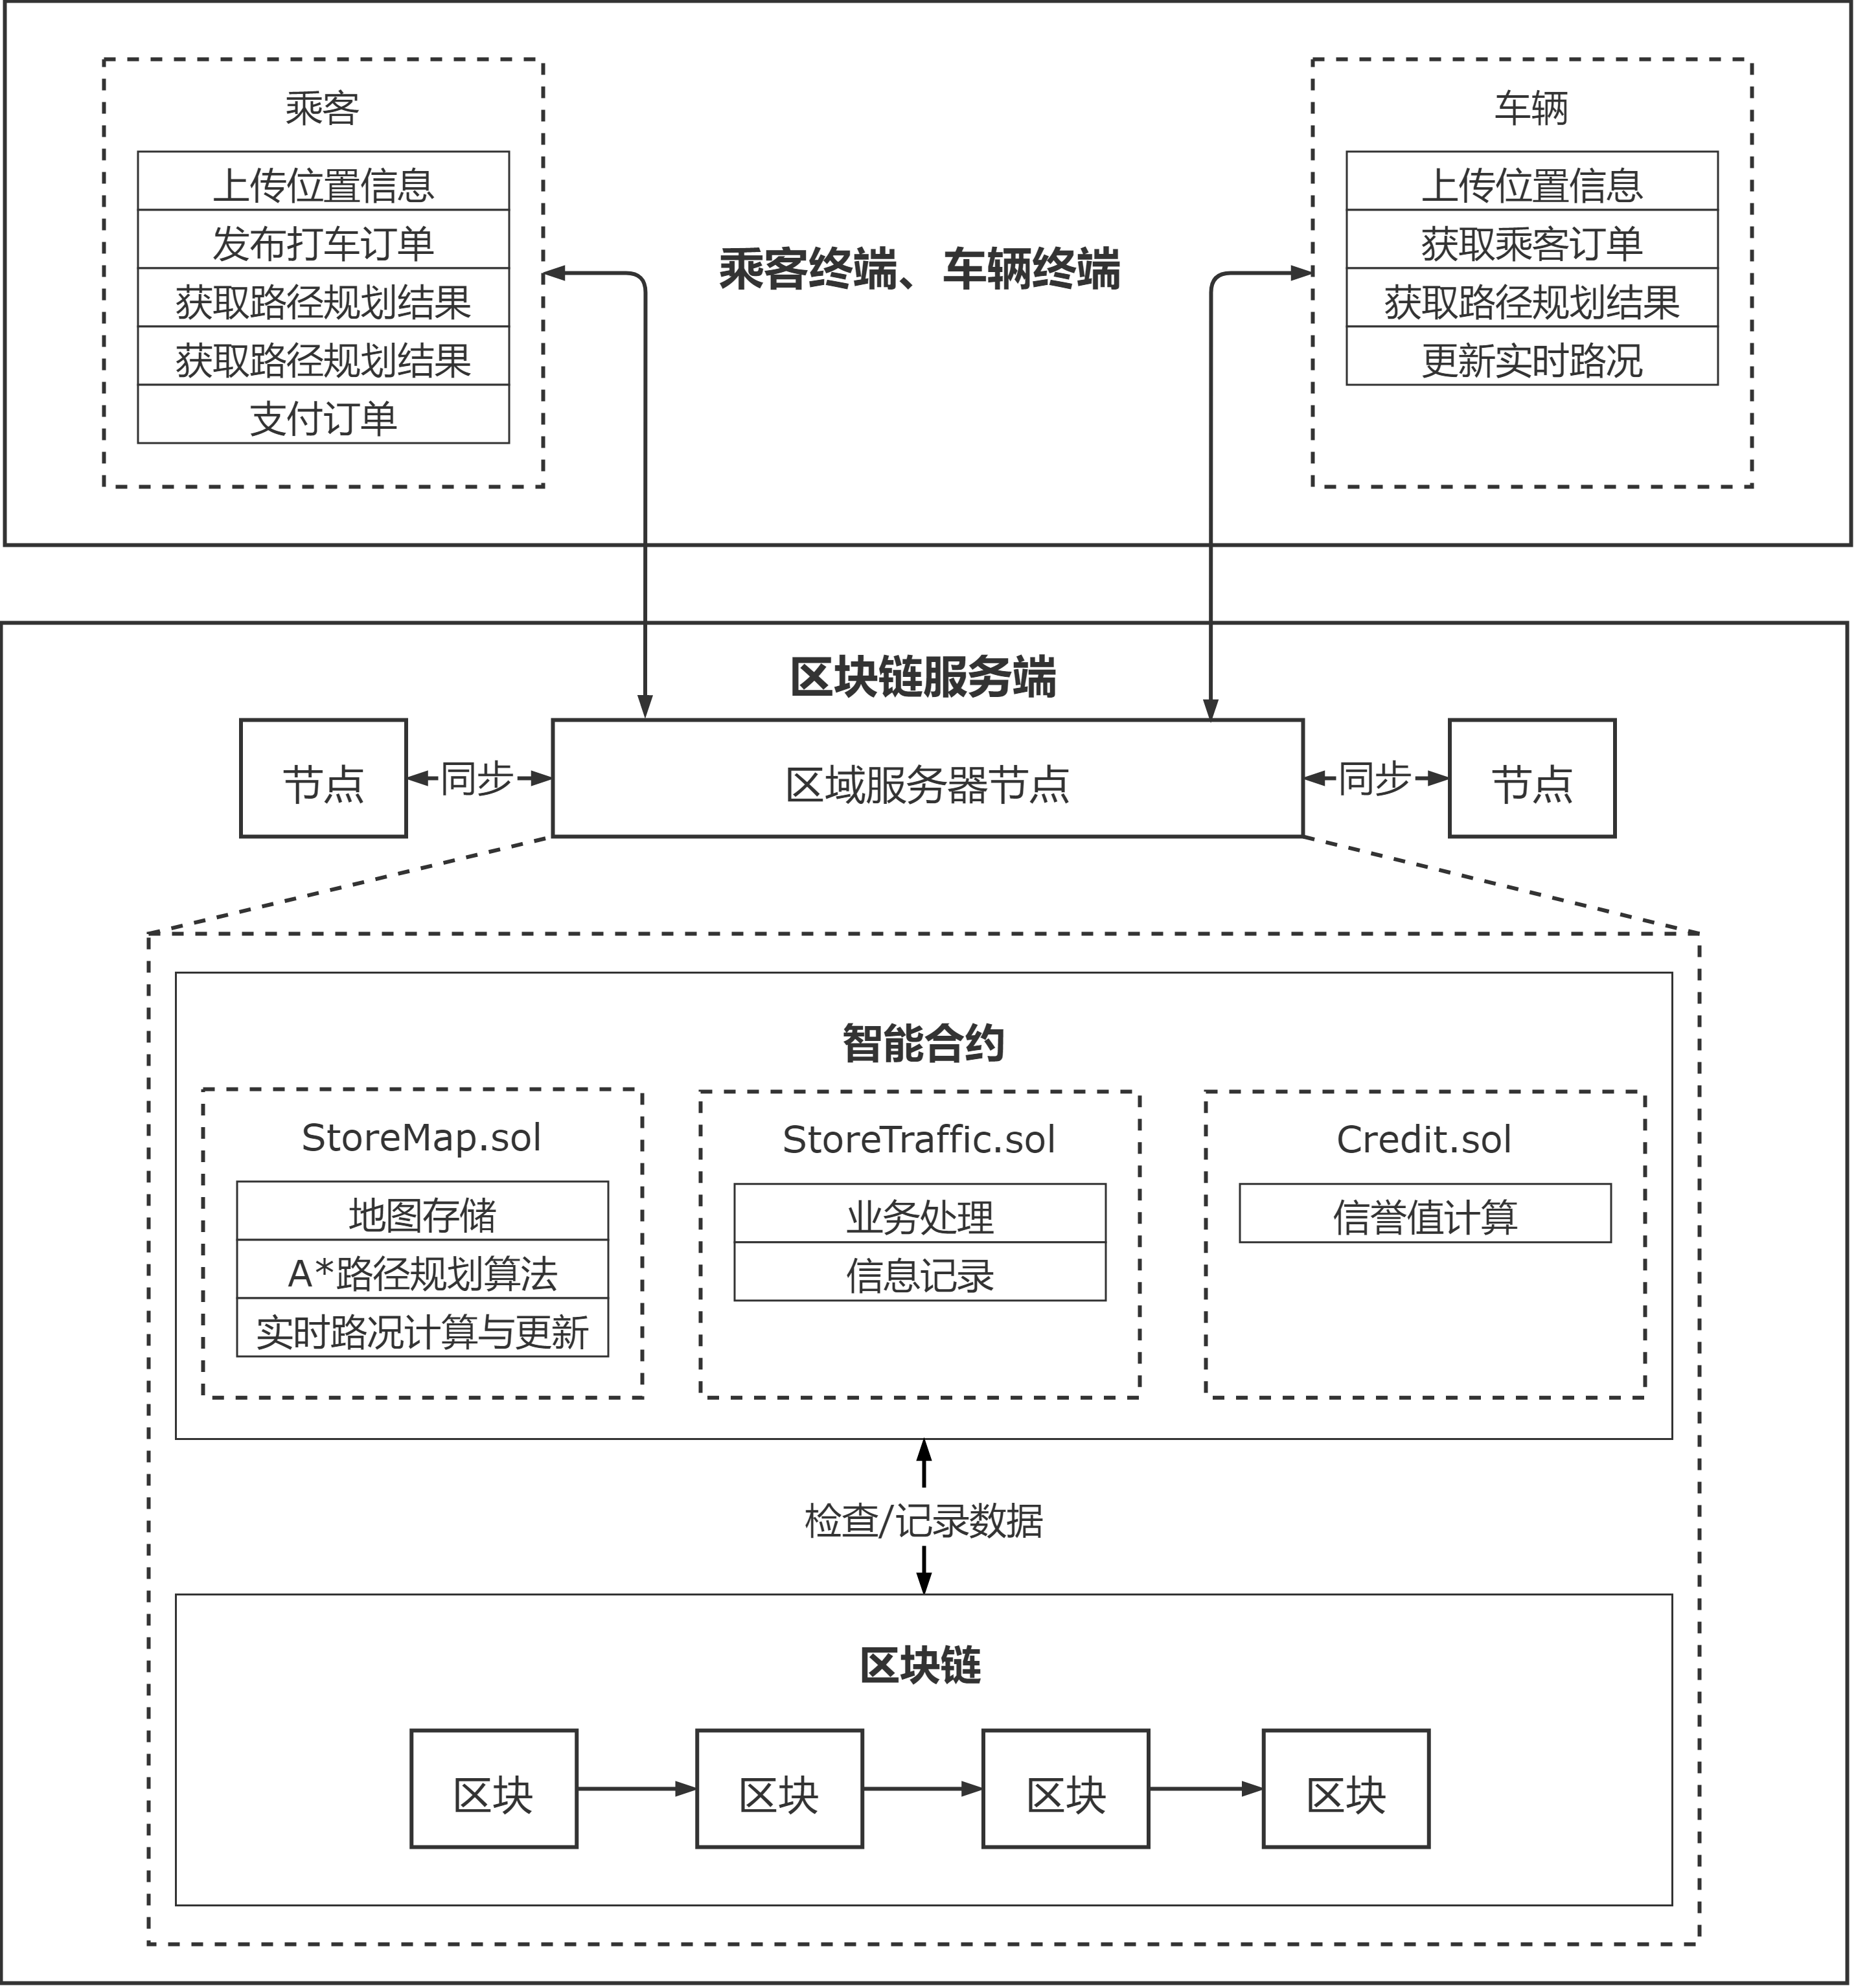
\includegraphics[width=0.7\textwidth]{undergraduate-thesis/images/sysstructure.png}
  \caption{基于区块链的出租车调度系统结构}
  \label{pic-sysstructure} % label 用来在文中索引
\end{figure}

图\ref{pic-sysstructure}是基于区块链的出租车调度系统结构示意图。本系统主要分为区块链服务器端和终端两部分,其中终端包括乘客终端与车辆终端。本系统去中心化,且为了保证身份信息的匿名性,乘客终端与车辆终端分别只与区块链交互,从而保证车乘之间不产生直接的信息交互。

\subsection{区块链服务器端}

区块链服务器端主要分区块链和智能合约两部分。

区块链部分主要实现数据存储功能,其存储交易相关数据与系统运行的地图数据。将数据存储在区块链上,能利用区块链数据的不可篡改性,保证交易安全有效,被需要时可以及时完成溯源。同时,当终端与区块链进行信息交互时,区域服务器节点也会与其他节点进行同步记录,保证在单个节点出问题时,其他节点能正常运行,而不受问题节点的影响,从而保证了数据的安全性。

智能合约部分主要负责对数据进行处理,它将区块链的功能从简单的记账拓展为复杂的事件响应、数据处理。本系统中共设计三个智能合约,其按功能被划分为地图合约(StoreMap.sol)、交通合约(StoreTraffic.sol)、信誉值合约(Credit.sol)。本文对地图合约进行了功能上的完善,为其补充了实时路况计算模块、并因此对地图合约里的A*算法进行了修改。下文将分别介绍这三个合约的功能。

1.地图合约主要完成地图存储、A*路径规划算法、实时路况计算与更新功能。该合约首先与地图上传脚本进行交互,将Geohash编码后的Json格式地图数据部署到区块链上,实现地图存储的功能。接下来,在终端的运行过程中,该合约根据终端发出的不同请求完成以下流程:在区块链上存储乘客、车辆位置信息;获取乘客的打车订单并运行车乘匹配算法为该订单调度车辆;将匹配结果告知乘客与车辆;为车辆规划出接乘客的路径并把结果返回给终端;为车辆规划出送乘客到目的地的路径并把结果返回给终端;根据送乘客的路径规划结果更新实时路况,并在区块链中以存储道路属性数据的形式存储路况。

2.交通合约主要完成业务处理、信息记录功能。在业务处理功能中,交通合约通过接收乘客的打车请求,实现按区域的车乘匹配,当车辆接到订单并选择接客后,交通合约修改车辆与乘客的状态为已载客、已乘车。信息记录功能则主要是对信息的处理过程,其接收到终端发来的车乘的位置信息、账户信息,同时也能修改车辆与乘客的载客与乘车状态,还能将乘客的支付状态告知给车辆,并且支持车辆退出系统的效果。

3.信誉值合约主要完成对车辆信誉值的计算。该合约把司机活跃度、车辆位置验证结果、车辆接单率、乘客主观评分四方面作为影响因子,进行计算,给出车辆的信誉值数据,使信誉值计算能综合车辆位置验证与交易评价两方面因素,更加全面合理。

\subsection{终端}

终端主要分为车辆终端与乘客终端。终端的实现方式分为脚本实现与浏览器实现。脚本实现方式的运行时间较浏览器实现更短。但浏览器实现能可视化观察到,在系统运行的各环节中,地图信息、车辆与乘客的位置、规划出的路径信息。本文工作重点为基于实时路况对A*算法进行改进,通过浏览器实现能更加直观给出本工作所得的动态路径规划效果,因此,本文主要通过浏览器实现的方式完成车辆终端与乘客终端的运行。

1.车辆终端通过web3接口与区块链服务端进行数据的交互,这些数据包括:在前端用于展示的地图数据、可视化的位置与路径规划结果信息数据;向区块链服务端发送自己的位置、账户信息,发送自己是否接客的信息;向区块链服务端发送信息,用于调用路径规划、实时路况计算等过程;从区块链服务端中获取打车订单信息,获取乘客支付信息。

2.乘客终端通过web3接口与区块链服务端进行数据的交互,这些数据包括:在前端用于展示的地图数据、可视化的位置与路径规划结果信息数据;向区块链服务端发送自己的位置、账户信息,发布打车订单,发送支付完成的信息;从区块链服务端中获取接到订单的车辆信息。

\section{传统A*算法与实时路况}

\subsection{传统A*算法的工作原理}
\label{A*Reason}

A*算法是一种在静态的路网中求解最短路径的直接搜索方法。该算法将Dijkstra算法和广度优先算法相结合,利用启发式函数寻找距起点代价最小的终点,从而规划出一条最短路径。该算法常被用于在地图中进行全局路径规划,也常常用于游戏中虚拟角色的移动计算。

A*算法将区域划分为小格,每个小格代表一个节点。A*算法以起点为中心,辐射性搜索周围的邻居节点,并计算每个节点的总距离代价,寻找代价最小的点继续移动,直至寻找到终点。针对节点n,A*算法将耗散函数、启发函数同时整合进公式\ref{cal-Astar}中,计算该节点的距离代价。
\begin{equation}
    F(n)=G(n)+H(n)
\label{cal-Astar}
\end{equation}

F(n)代表节点n对应的总距离代价;G(n)是耗散函数,它代表从起点到节点n,该路径已经花费掉的所有代价,也即从起点到节点n的实际距离;H(n)是启发函数,它代表从节点n到终点,预估将要花费的代价。

对第n个节点来说,由于耗散函数G(n)代表它从起点到该点的实际距离,因此G(n)的值一般为固定值,它的计算方式也是固定的。启发函数H(n)的选取方式则相对多样。在A*算法中,启发函数的选取也是至关重要的一环。启发函数的作用是预估从节点n到终点所需的距离代价。

在公式\ref{cal-Astar}中,如果令H(n)=0,则F(n)=G(n),此时总距离代价完全由耗散函数G(n)控制,则A*算法将退化为Dijkstra算法。在这种情况下,尽管最终仍能寻到起点与终点之间的最短路径,但消耗的时间和内存空间都将较H(n)≠0时有所增加。

在公式\ref{cal-Astar}中,如果令G(n)=0,则F(n)=H(n),此时总距离代价完全由启发函数H(n)控制,则A*算法将退化为广度优先搜索。这种情况将导致算法进行盲目的搜寻,其不注重结果的可能位置,而是彻底搜索整个图,尽管它也能给出规划结果,但它找出的结果是单一的,有时甚至找不到最短路径,且消耗的时间和内存空间也较G(n)≠0时更多。

因此,给G(n)和H(n)分配适当的权值,从而令A*算法有一个合适的评估函数F(n),是非常关键的。一般在计算时给G(n)和H(n)分配的比例是1:1,本文中也沿用此评估函数。

在计算启发函数H(n)时,常常有以下几种计算方法:

\begin{enumerate}
    \item 欧几里得距离(Euclidean distance):
        \begin{equation}
            D(M,N)=\sqrt[2]{ (x_{2}-x_{1})^{2} + (y_{2}-y_{1})^{2}} 
        \label{Eu-dis}
        \end{equation}

        欧几里得距离也称欧氏距离。假设待计算的两点坐标为:M(x1,y1)、N(x2,y2),则该计算方式得出的结果D(M,N)是两个地理位置之间的直线距离,如公式\ref{Eu-dis}。
        
        该距离计算公式适用于能朝任何方向移动的路径规划过程。
    
    \item 曼哈顿距离(Manhattan Distance):
        \begin{equation}
            D(M,N)=\left | x_2-x_1 \right | + \left | y_2-y_1 \right |
            \label{Man-dis}
        \end{equation}
        
        假设待计算的两点坐标为M(x1,y1)、N(x2,y2),则该计算方式得出的结果D(M,N)是两个地理位置在标准坐标系上的绝对轴距总和,如公式\ref{Man-dis}。

        该距离公式适用于能朝上下左右四个方向移动的路径规划过程。
\end{enumerate}

% 空行有点点大惹,看看怎么减一减
% \vspace{-1cm}
\begin{figure}[ht]
  \centering
  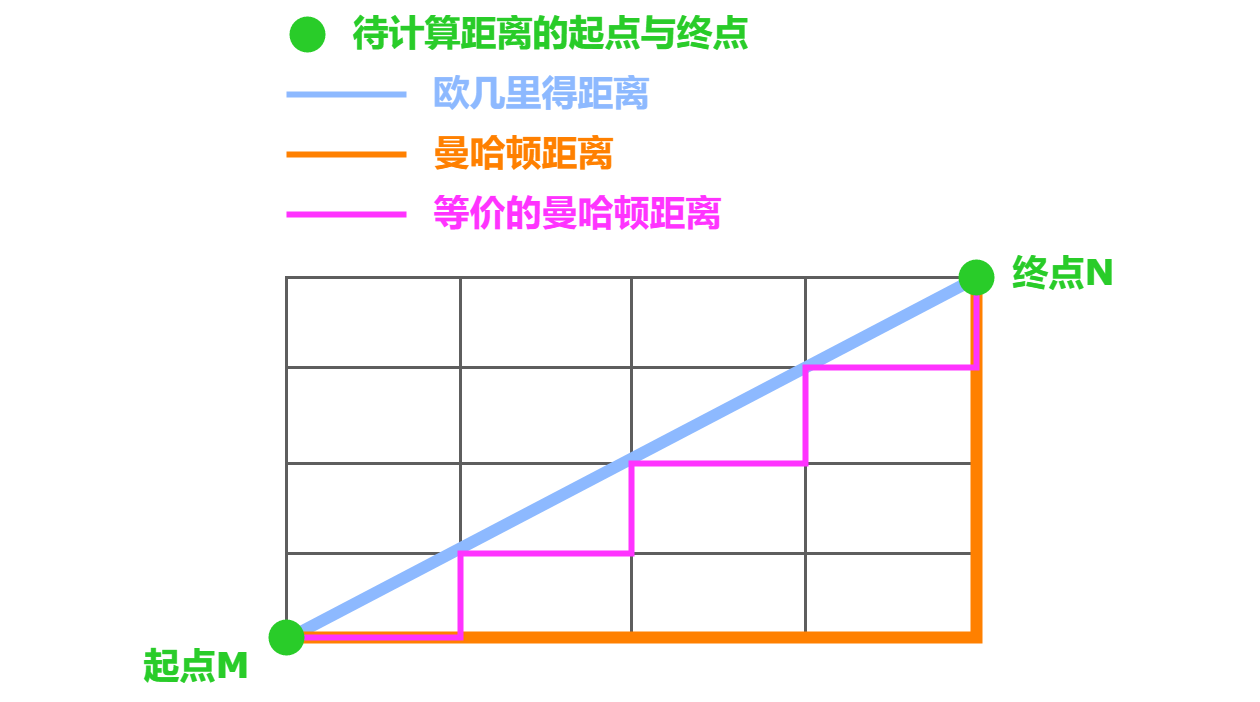
\includegraphics[width=0.5\textwidth]{undergraduate-thesis/images/EuDis_and_ManDis.png}
  \caption{欧几里得距离和曼哈顿距离示意图}
  \label{EuDisAndManDis} % label 用来在文中索引
\end{figure}

以一个3*4大小的方格区域为例,在该方格区域中分别使用这两种距离计算方法计算起点与终点间的距离,其各自规划出的路径如图\ref{EuDisAndManDis}所示。可以看到,用欧几里得距离规划路径时,由于欧几里得距离允许车辆向任何方式行驶,所以它直接按照蓝色斜线从起点前往终点;用曼哈顿距离规划路径时,它将按照方格边缘行驶,即只沿正南、正北、正东、正西方向计算路程,最终按照橙色折线或粉色折线从起点前往终点。

由于城市中的道路大多具有固定朝向,不存在行驶中的车辆能朝着任意方向运行的可能性。且在基于Geohash编码地图时,会将地图划分成不同区域的小方格,符合曼哈顿距离在计算时的沿方格边沿计算特性,因此在本出租车调度系统中,采取曼哈顿距离作为A*算法中的启发函数。

\begin{figure}[ht]
  \centering
  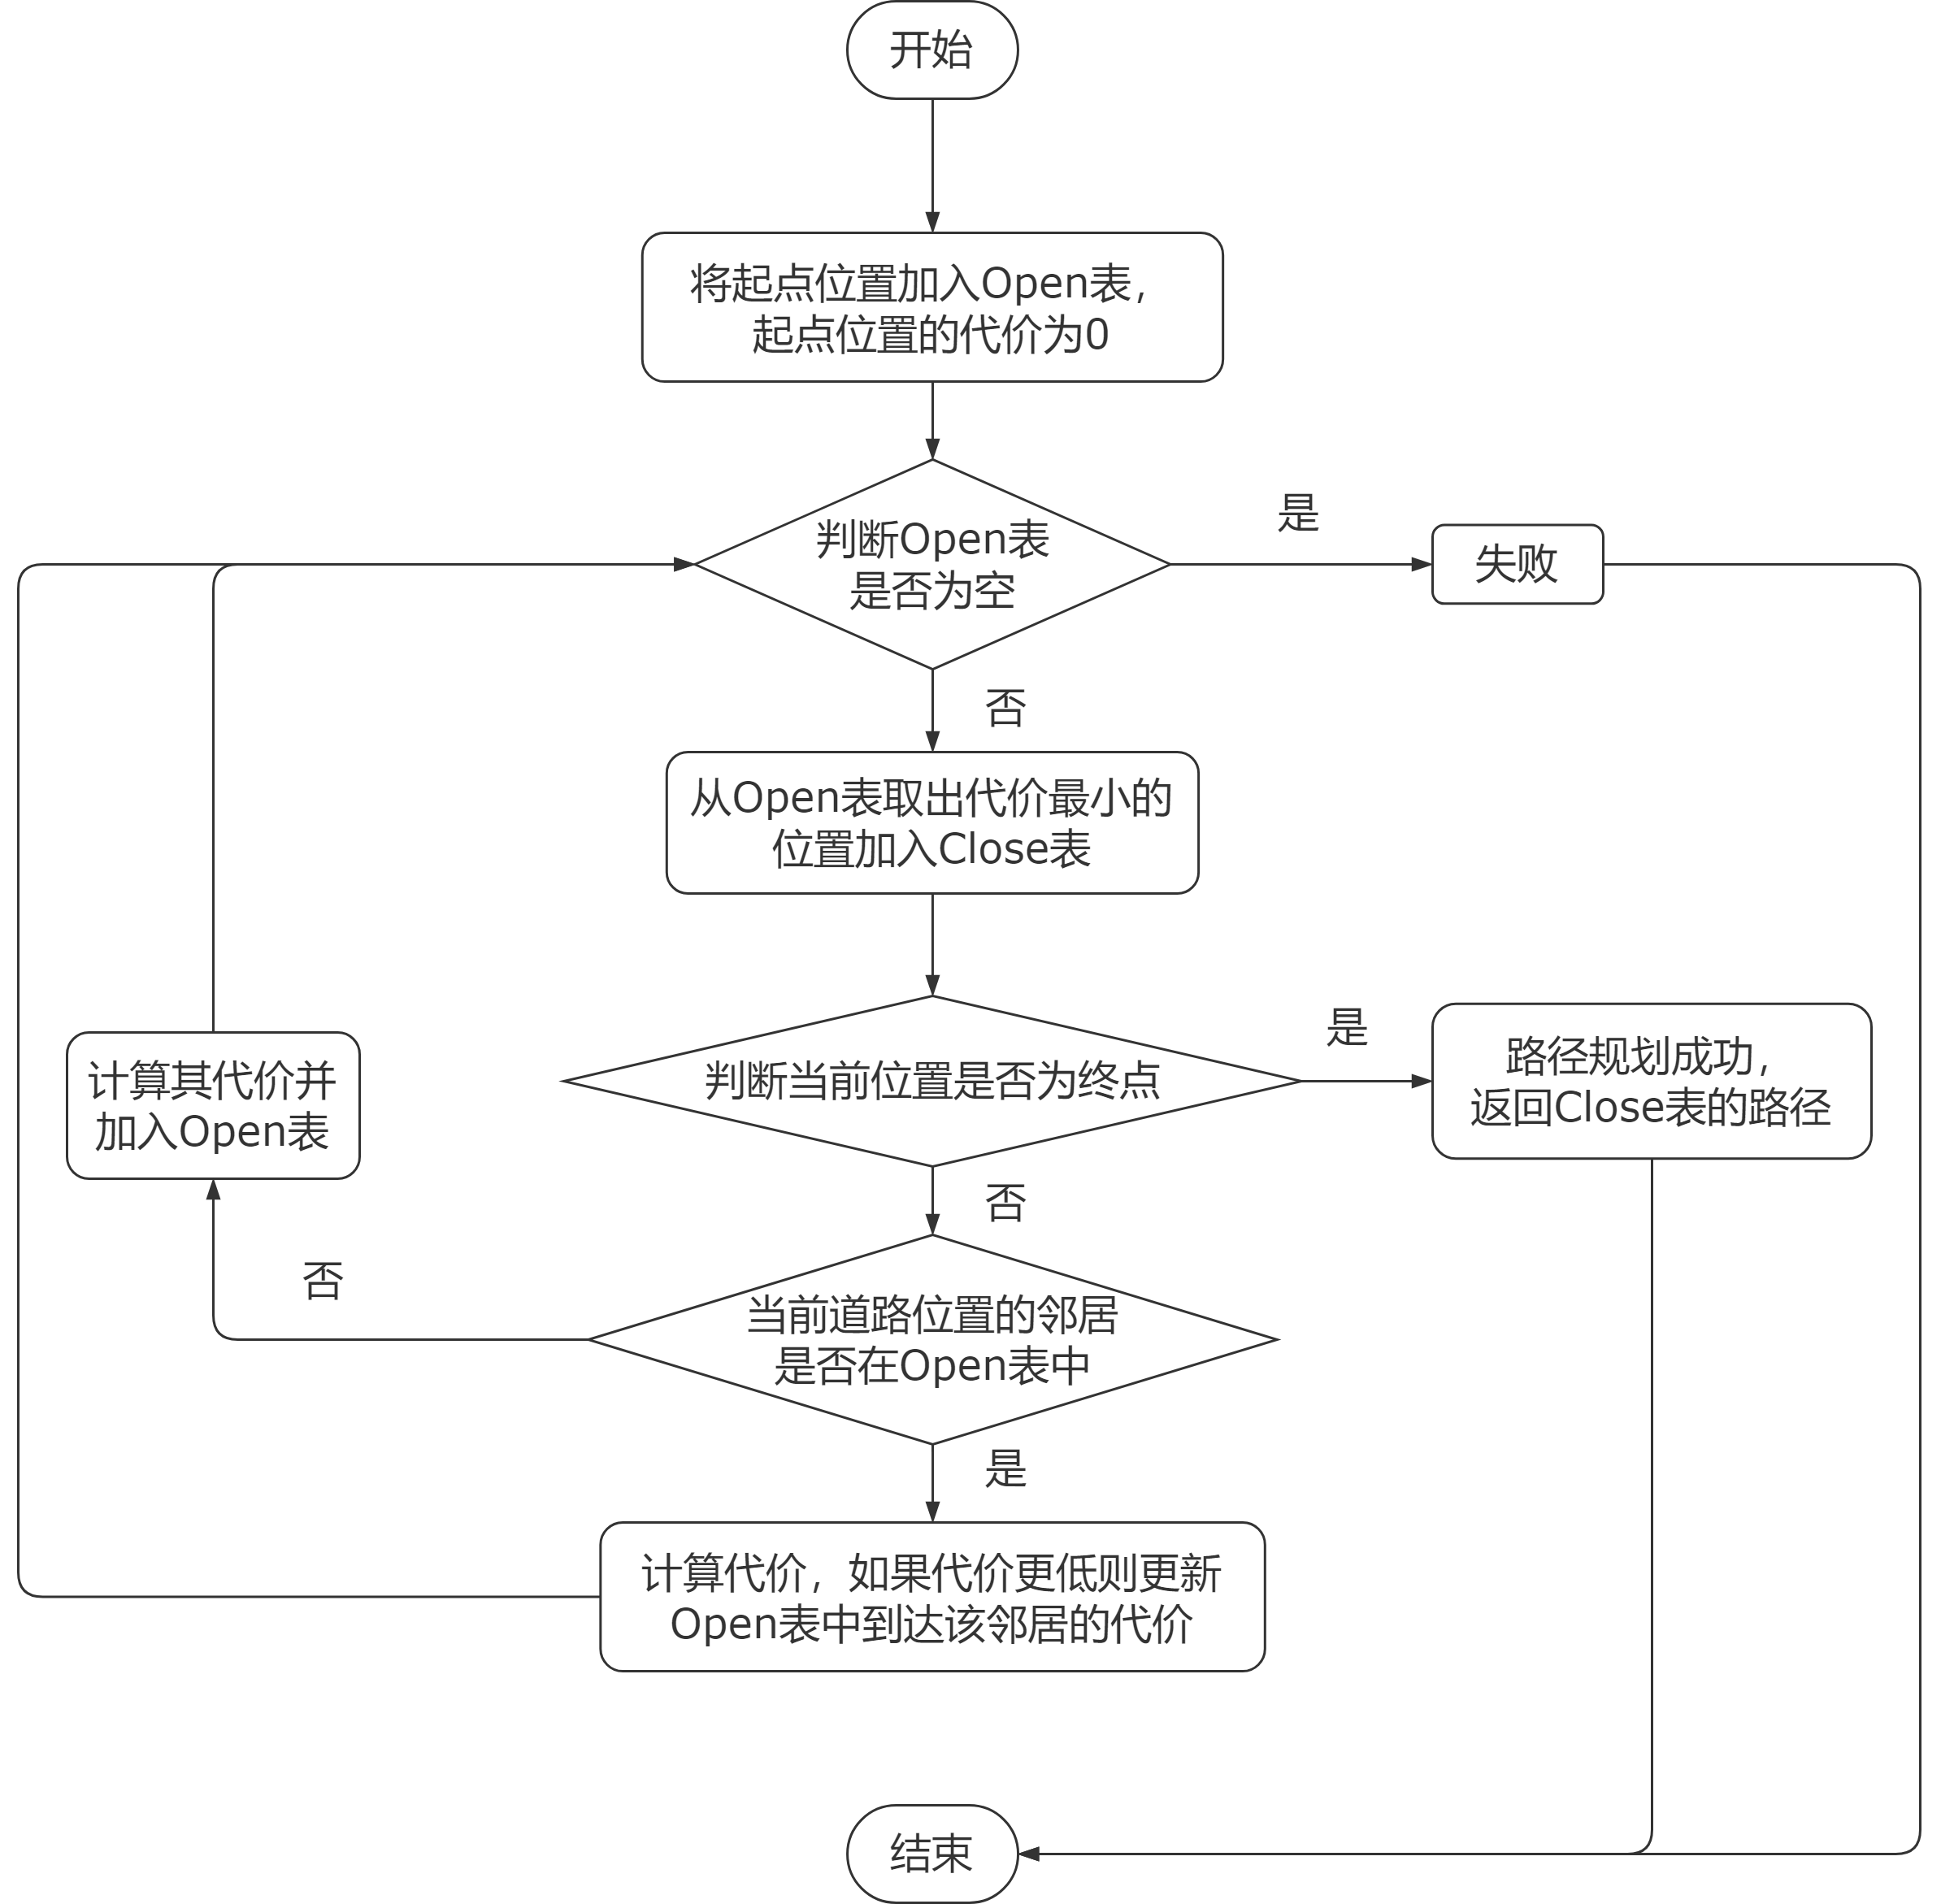
\includegraphics[width=0.65\textwidth]{undergraduate-thesis/images/Astar_Workway.png}
  \caption{A*算法流程图}
  \label{AstarWorkWay} % label 用来在文中索引
\end{figure}

如图\ref{AstarWorkWay}所示,A*算法在运行时的关键在于维护Open表和Close表、计算总距离代价F。设当前节点为P,则P点的每一个邻居$p_i$都存在其总距离代价F($p_i$)。Open表中记录所有与P相邻的点,它集中了节点P有可能前往的所有下一个节点;Close表中记录已走过的点,它集中了目前的路径规划已走过的道路,这意味着Close表中的点一定是最终规划出的最短路径中会经过的点。对节点P来说,计算完它邻居$p_i$的总距离代价F($p_i$)后,从所有的F($p_i$)中找到最小值F($p_{min}$)及其对应的点P$_{min}$点,将P$_{min}$点加入Close表中,然后把当前节点P移至节点P$_{min}$,再去计算P$_{min}$点的邻居的总距离代价F,从而从起点一层层向外扩散移动,直至寻找到终点。一旦A*算法寻找到终点,Close表中存放的点序列就是此次算法运行所规划好的运行路径。

\begin{figure}[!ht]
  \centering
  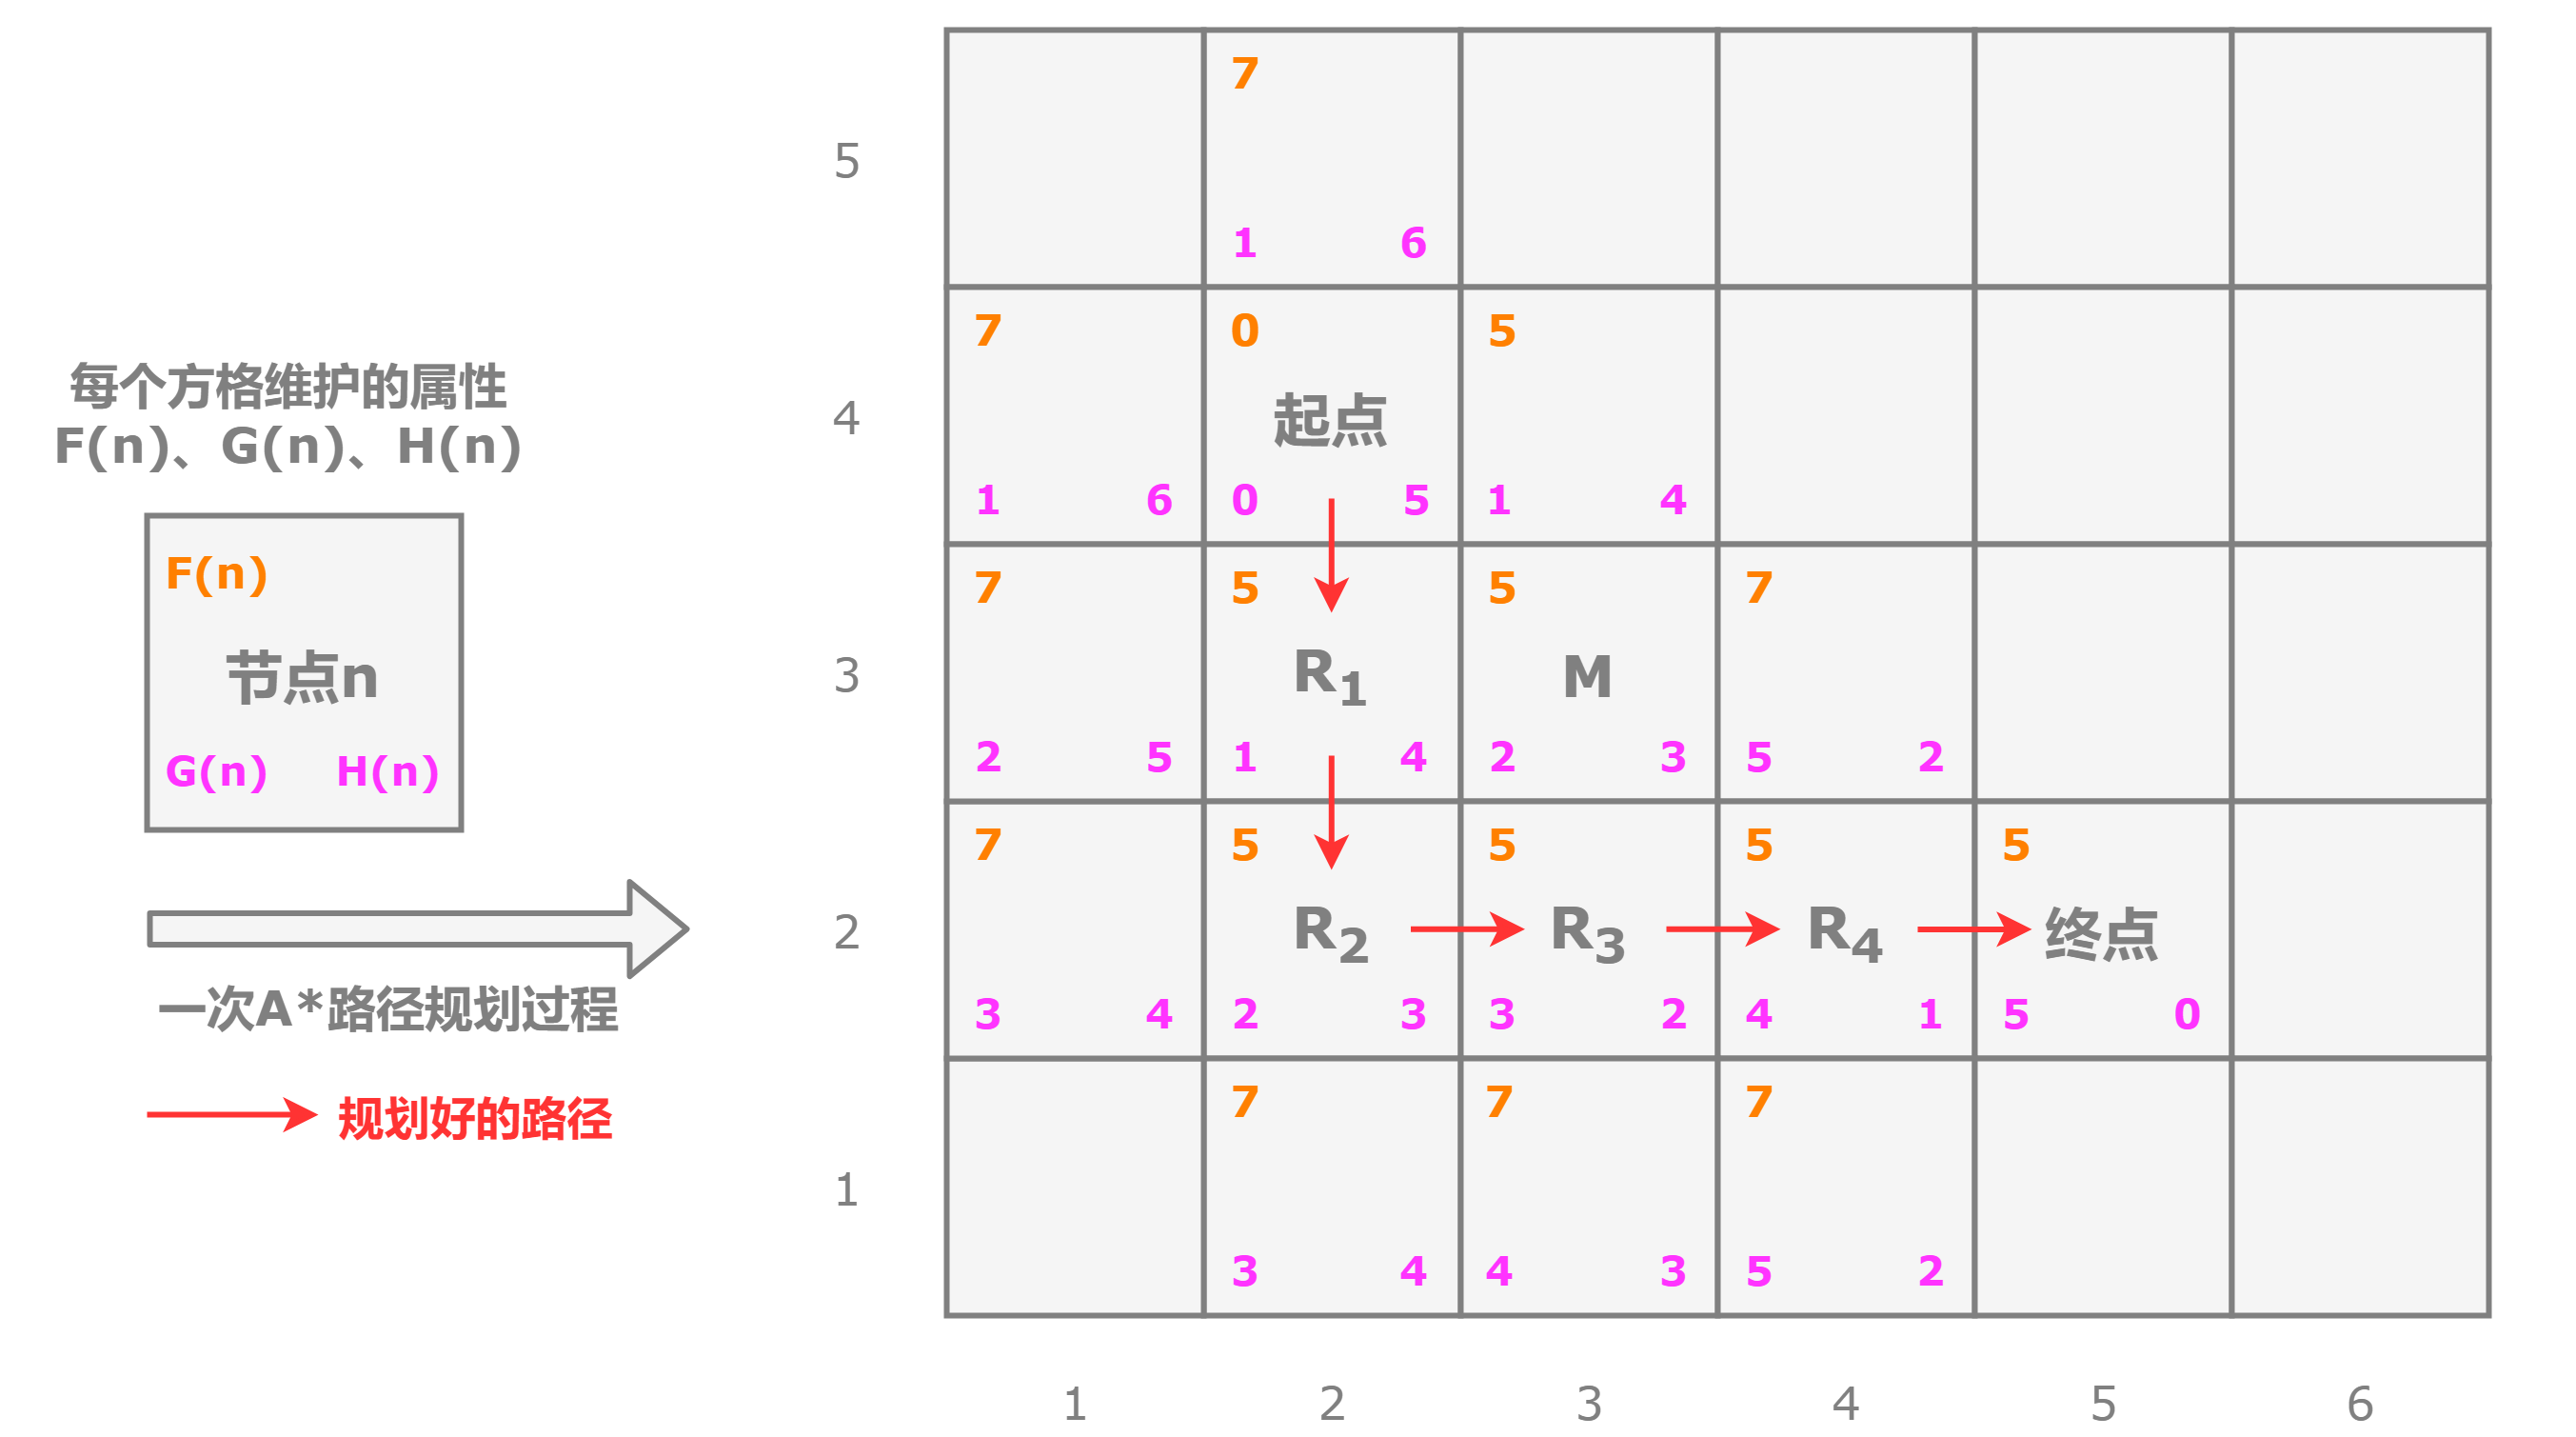
\includegraphics[width=0.8\textwidth]{undergraduate-thesis/images/Astar_Fn.png}
  \caption{A*算法示例}
  \label{AstarFn} % label 用来在文中索引
\end{figure}

图\ref{AstarFn}是A*算法运行过程的简单示意图。在该示意图中,假设一辆车需要从起点驶向终点,且该车辆只能朝上下左右四个方向驾驶,每个方格为正方形,边长为单位长度1,在计算启发函数H(n)时使用曼哈顿距离,并要求,如果计算出的总距离代价F相同,则优先朝下侧移动,再朝右侧移动,再朝上侧移动,最后朝左侧移动。

在上述场景中,结合图\ref{AstarFn},A*算法为起点与终点规划路径时的运行过程如下:

\begin{enumerate}
    \item 从起点到$R_1$点(第1轮):将起点位置加入Open表,然后从起点一圈圈向外寻找。首先找到的是起点的上下左右四个邻居方格,将它们加入Open表里,将起点加入Close表。分别计算这四个邻居方格的总距离代价F,得出起点下侧和右侧邻居的F同时最小,则按照假设,车辆向下侧移动,移至$R_1$点位,同时将$R_1$加入Close表中。
    \item 从$R_1$点到$R_2$点(第2轮):在$R_1$点位搜索邻居方格,发现起点作为$R_1$的上侧点位,实际上已经进入Close表中,因此,将$R_1$的左、右、下侧三个点加入Open表,作为邻居方格,并分别计算这三个邻居方格总距离代价F,得出$R_1$下侧和右侧邻居的F同时最小,按照假设,车辆向下侧移动至$R_2$点位,将同时将$R_2$加入Close表中。
    \item 从$R_2$点到$R_3$点(第3轮):在$R_2$点位搜索邻居方格,将$R_2$点位的左、右、下侧三个方格作为邻居方格,计算得到移动的下一个位置是$R_3$,将车辆移至$R_3$。
    \item 从$R_3$点到$R_4$点(第4轮):在$R_3$点位搜索邻居方格,将$R_3$的上、下、右侧三个方格作为邻居方格加入Open表中计算代价F。要注意的是,由于在第2轮中,邻居方格M已经被加入Open表,计算过一次总距离代价F,在本轮中,将对M重新计算总距离代价,所得代价较第2轮中计算的结果更高,因此不更新M在Open表中对应的F值。计算得到本轮移动的目的地为$R_4$。
    \item 从$R_4$点到终点(第5轮):在$R_4$点搜索邻居方格,将$R_4$的上、下、右侧三个邻居列入本轮的总距离代价计算过程中,结果是移至终点的F最小,因此将终点加入Close表,车辆的当前位置移动为终点,则路径规划成功,算法运行结束。
\end{enumerate}

在此例中,A*算法寻得的路径为:起点 -> $R_1$ -> $R_2$ -> $R_3$ -> $R_4$ -> 终点。

\subsection{传统A*算法与实时路况结合的必要性}

在章\ref{A*Reason}中,结合具体例子可知,A*算法有以下特性:

特性1:基于栅格法分割地图。

特性2:只关注静态的地图和方格间的距离本身。

针对A*算法的特性1,本文中的出租车调度系统基于Geohash编码的矢量地图数据,其借助Geohash编码将地图分成了大小相同的多个小方格,并且为每个地图中的运行道路都事先计算好用于反映路段距离的成本(cost)属性,该属性以米为单位。同时,本系统采用的启发函数是曼哈顿距离,符合地图数据和A*算法的方格特性。

针对A*算法的特性2,在真实的行车过程中,司机选择行驶道路的考虑因素是多方面的。路径长度是一个重要的考虑因素,同时,路况信息是另一个重要的考虑因素。路况信息能实时反映区域内的交通拥堵情况,便于司机估算前往目的地的用时,从而为司机提供一个最快捷、最通畅的最佳行驶路线。A*算法能够在起点和终点间搜寻到一条路程最短的规划路线,因此,在此基础上,引入实时路况的影响因子,才能更加真实地模拟汽车运行轨迹。

本文将在章\ref{A*New}中给出一种结合实时路况的改进A*算法设计。

\section{结合实时路况的改进A*算法}
\label{A*New}

\begin{figure}[!ht]
  \centering
  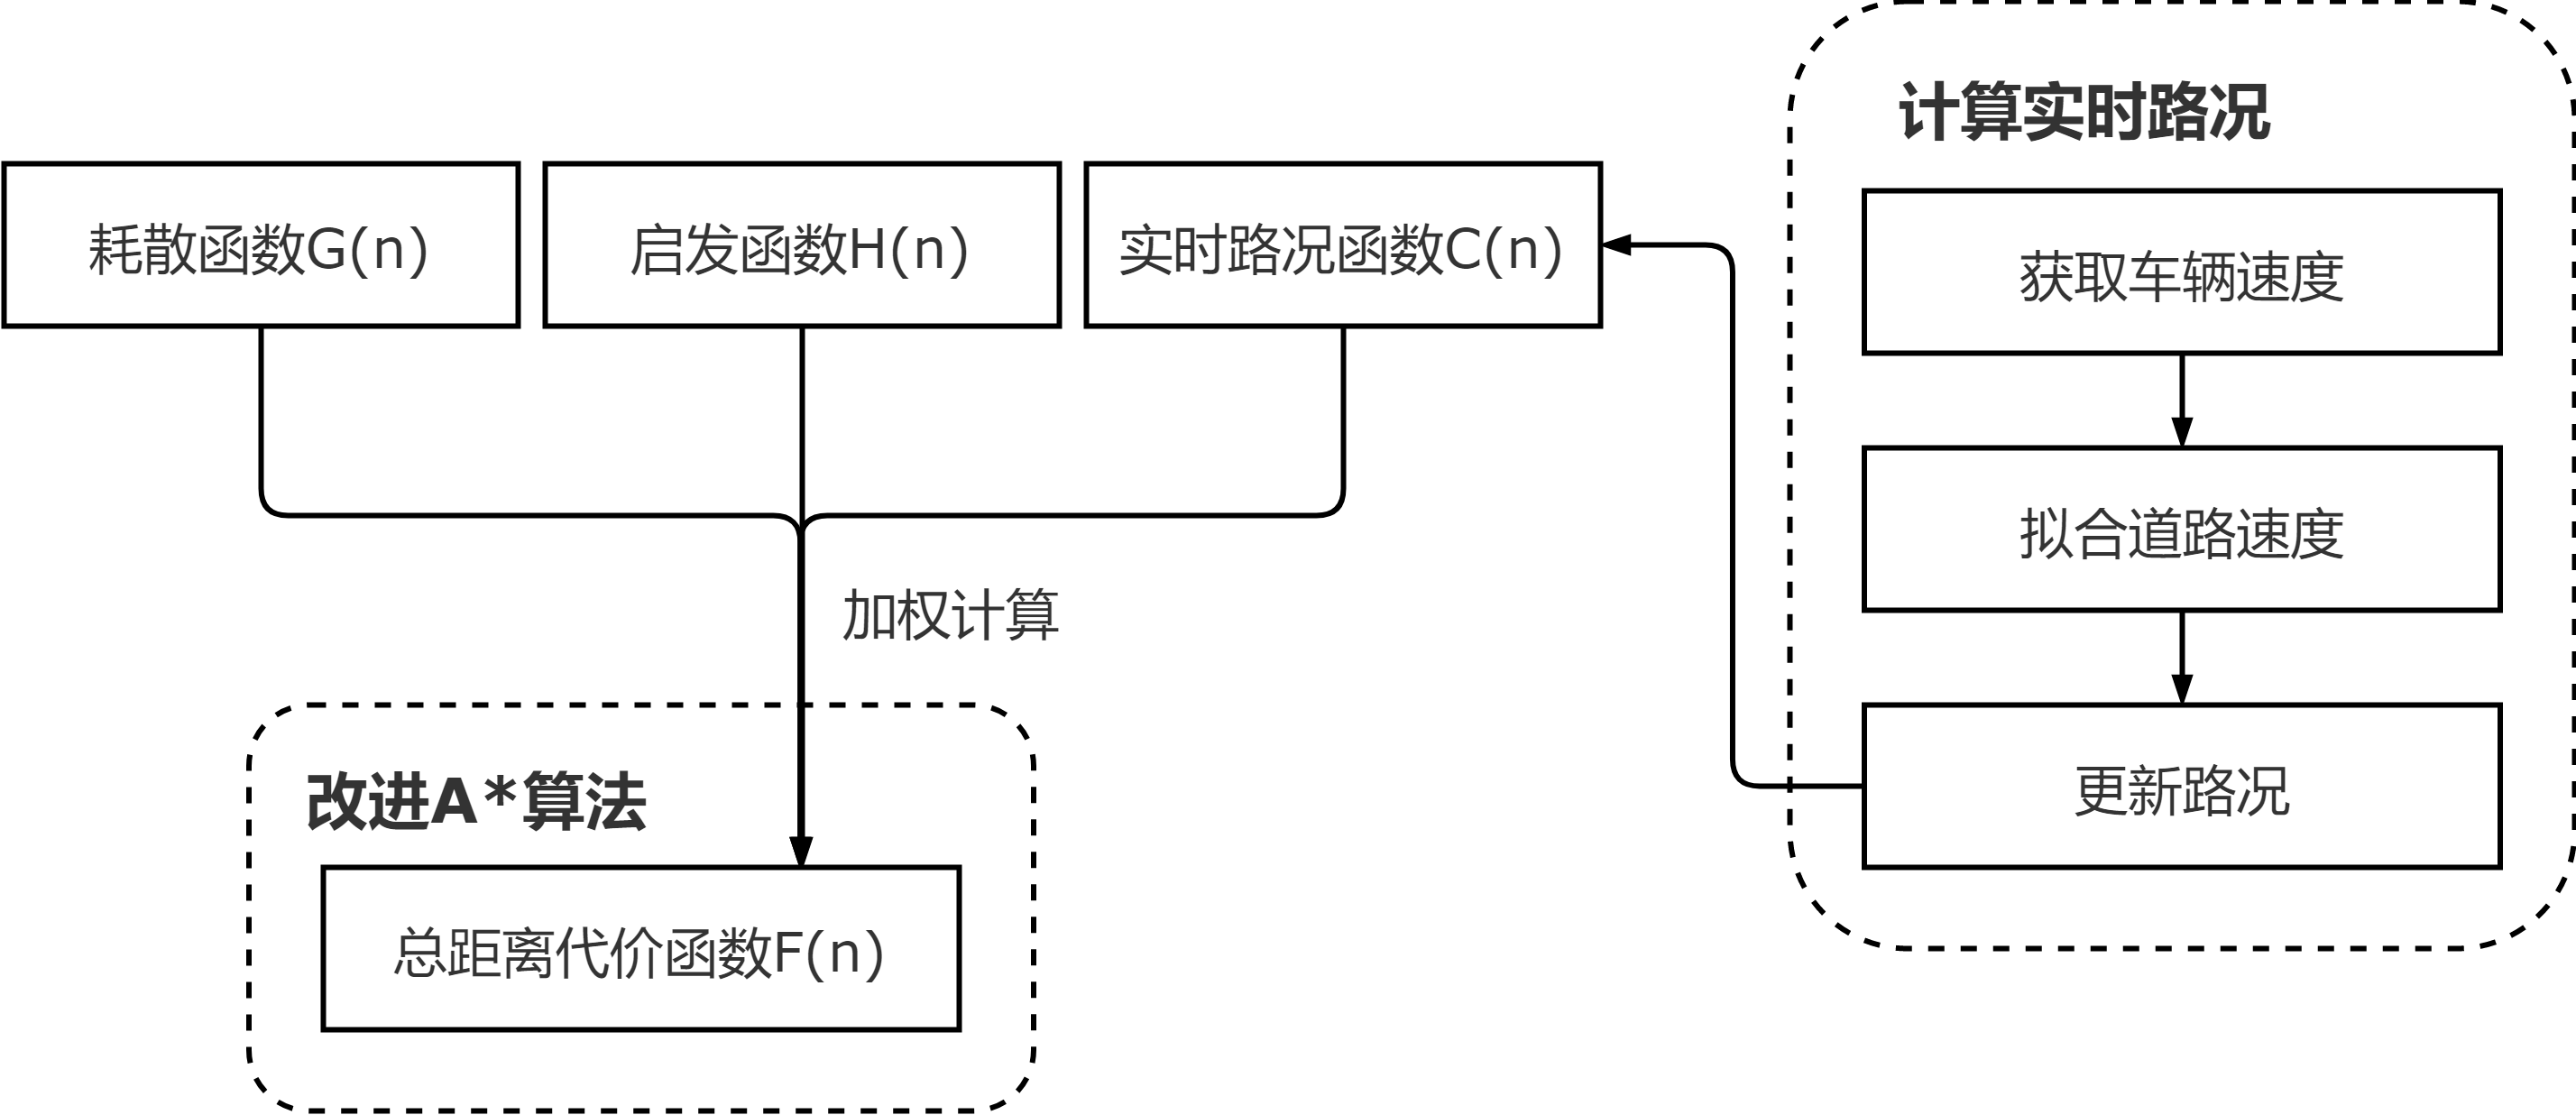
\includegraphics[width=0.7\textwidth]{undergraduate-thesis/images/Astar_new.png}
  \caption{结合实时路况的改进A*算法示意图}
  \label{newAstarIdea} % label 用来在文中索引
\end{figure}

本节设计了一种结合实时路况的改进A*算法,如图\ref{newAstarIdea}所示,本算法主要分为计算实时路况、改进A*算法两部分,在计算实时路况部分需要获取车辆速度、拟合道路速度、更新路况;在改进A*算法部分需要改动总距离代价函数F(n)的计算方式。

\subsection{符号与假设}

\begin{table}[ht]
  \linespread{1.5}
  \zihao{5}
  \centering
  \caption{符号表}\label{currentPathSymbols}
  \begin{tabular}{cc} 
  \toprule
    符号 & 含义 \\ 
  \hline
    $Round_i$ & 车辆运行的第i个轮次 \\
    $Vehicle_j$ & 第j辆车的名称 \\
    $Speed_j$ & 第j辆车的速度 \\
    $Distance_j$ & 第j辆车的行驶距离 \\
    $Time_j$ & 第j辆车的行驶时间 \\
    $V_{default}$ & 当前路段的限速,是道路的固定属性,永远不变 \\
    $V_{path,i}$ & 第i轮中,由n辆车拟合出的道路速度 \\ 
    $V_{History,i}$ & 第i轮中,道路的历史路况,是道路的属性 \\
    $V_{Current,i}$ & 第i轮中,道路的当前路况,是道路的属性 \\
    $V_{Fact,i}$ & 第i轮中,道路的实时路况,是道路的属性 \\
    F(n) & 节点n对应的总距离代价 \\
    G(n) & 节点n对应的耗散函数 \\
    H(n) & 节点n对应的启发函数 \\
    C(n) & 节点n对应的实时路况成本函数 \\
  \bottomrule
  \end{tabular}
\end{table}

章节\ref{A*New}中所用到的所有符号及其含义如表\ref{currentPathSymbols}中所示。其中,道路的历史路况$V_{History,i}$表示第$Round_{i-1}$轮计算出的实时路况,其在第$Round_{i-1}$轮中是实时路况,在第$Round_{i}$轮中成为历史路况;道路的当前路况$V_{History,i}$表示第$Round_{i}$轮中,由车辆拟合出的速度所代表的道路当前路况;道路的实时路况$V_{Fact,i}$表示第$Round_{i}$轮中,根据道路的历史路况和当前路况加权计算出的道路的实时路况,这是改进后的A*算法在进行路径规划时的主要依据之一。

%这图好像有点黑...
\begin{figure}[ht]
  \centering
  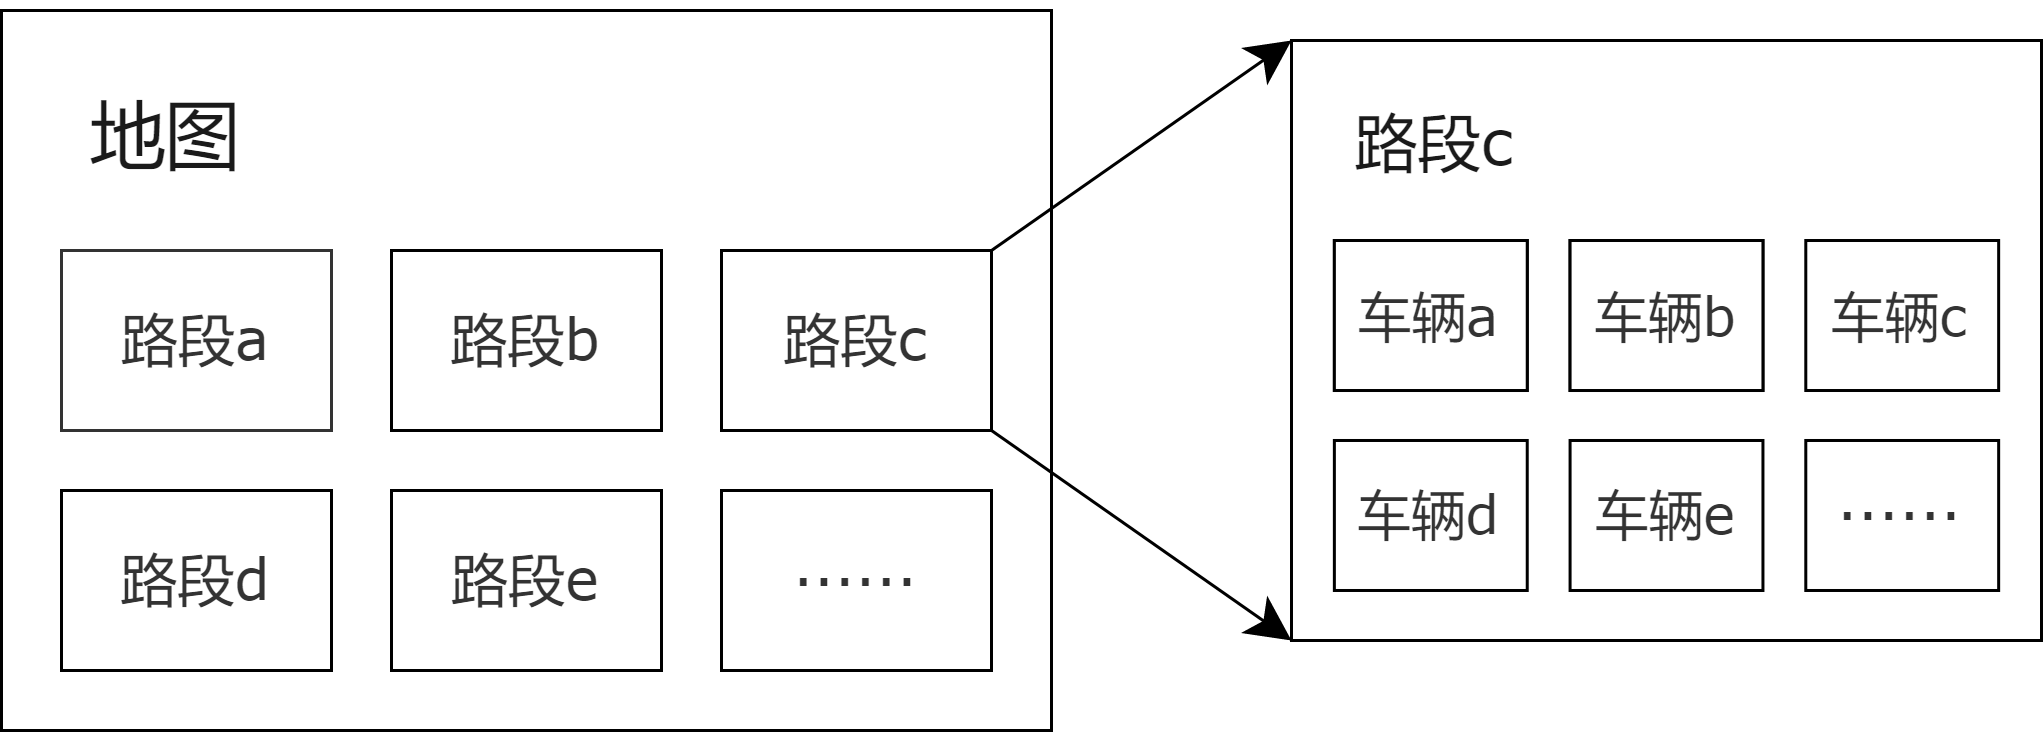
\includegraphics[width=0.7\textwidth]{undergraduate-thesis/images/MapPathVehicle.png}
  \caption{地图、路段、车辆的关系示意图}
  \label{mappathvehicle} % label 用来在文中索引
\end{figure}

图\ref{mappathvehicle}给出了本文系统中的三要素(地图、路段、车辆)关系。一份地图里会有$x(x>0)$个路段,在结合改进A*算法之后的出租车调度系统中,每个路段上会存在$y(y\ge 0)$辆车。

假设当前路段上存在运行中的车辆,假设一共有$n$辆车,这$n$辆车的起点为路段起点,这$n$辆车的终点为路段终点。这$n$辆车在当前路段运行一次,称为``车辆运行的第1个轮次”,在本轮运行完毕之后,这$n$辆车立刻回到原起点,等待下一轮运行,成为``车辆运行的第2个轮次”,这样循环往复,一共运行$m$轮。在这$m$轮的运行中,旧轮次的路况将成为影响新轮次路况计算的因素。

\subsection{实时路况的计算思路}
\label{subsection-calPathSituation}

每个城镇都包含成千上万条道路,随着城镇车辆的增加,道路拥堵现象已经成为普遍现象,尤其是在人群上下班的高峰期,道路拥堵的严重程度尤为突出。本节设计了一种计算实时路况的算法。

首先,是需要获取车辆速度。在获取车辆速度时,最常规的做法即利用车辆的运行距离$Distance$和运行时间$Time$计算车辆的速度。对$Round_k$中的第i辆车辆来说,其运行速度计算过程如公式\ref{calvspeed}。

\begin{equation}
    Speed_i = \frac{Distance_i}{Time_i} 
\label{calvspeed}
\end{equation}

其次,是需要拟合道路速度$V_{path}$。对道路速度的拟合计算,需要考虑路段中无车、有车两种情况。在道路无车时,如第一次初始化出每条道路时,没有车辆能影响当前道路的拟合速度,因此,道路的速度$V_{path}$等于其本身的固定属性限速$V_{default}$;在道路有车时,车辆速度将在不同程度上影响道路速度$V_{path}$,假设此时道路上一共有$n$辆车,第$i$辆车命名为$Vehicle_i$,其运行速度为$Speed_i$,则道路速度$V_{path}$的计算公式为取这些车辆的均值,如公式\ref{calpathSpeed}。
\begin{equation}
V_{path} =
  \left\{\begin{matrix}
  V_{default} & ,When\enspace there\enspace are\enspace no\enspace vehicles\enspace on\enspace the\enspace road. \\
  \frac{1}{n} {\sum_{i=1}^{n}Speed_i} & ,When\enspace there\enspace are\enspace vehicles\enspace on\enspace the\enspace road.
\end{matrix}\right.
\label{calpathSpeed}
\end{equation}

最后,需要按照前两步计算的内容,更新路况。其中,需以道路速度为量化数据代表路况。此时已通过$n$辆车的速度,综合起来计算得出了道路速度$V_{path}$。每个路段维护表\ref{currentPathSymbols}中的$V_{History}$、$V_{Current}$、$V_{Fact}$三个属性字段。在当前路段中,每轮有$n$辆车在道路上运行,一共运行$m$轮。

\begin{figure}[ht]
  \centering
  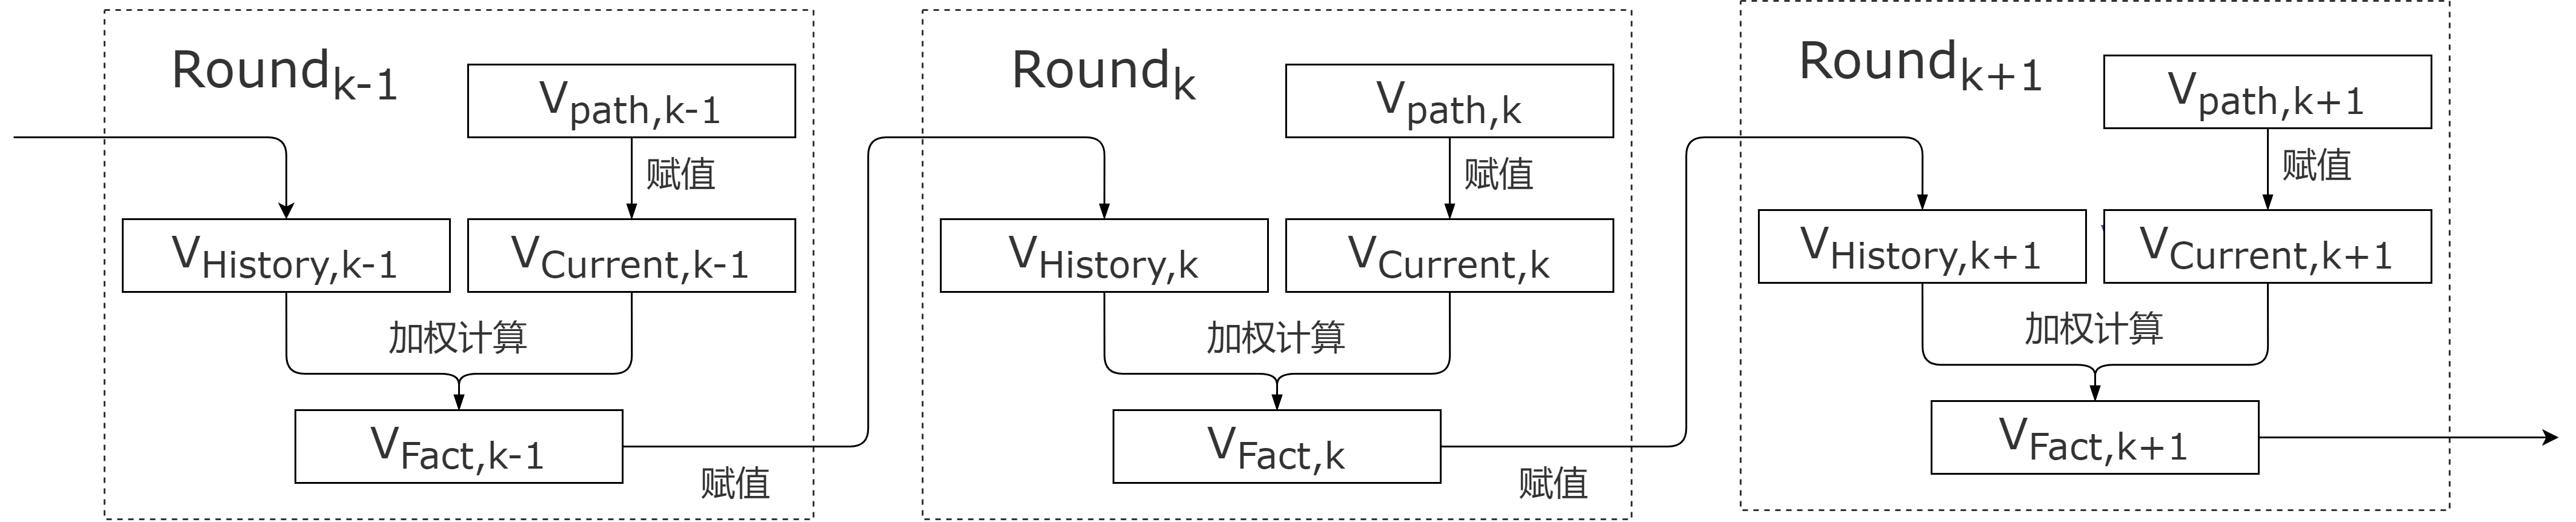
\includegraphics[width=1\textwidth]{undergraduate-thesis/images/calFactPathSituation.png}
  \caption{实时路况的迭代过程}
  \label{calFactPathSituation_pic} % label 用来在文中索引
\end{figure}

路况的计算是一个不断迭代的过程。如图\ref{calFactPathSituation_pic},设目前系统运行到了第$k$轮,则上一轮是第$k-1$轮,下一轮是第$k+1$轮。在上一轮中,路段的速度计算为$V_{Fact,k-1}$,本轮中路段的速度计算为$V_{path,k}$。则$V_{History,k}$、$V_{Current,k}$属性字段与路段速度的关系如公式\ref{calpathSituation}。该道路上一轮的通行速度$V_{Fact,k}$可以作为当前轮次的历史路况$V_{History,k}$。
\begin{equation}
    \left\{
    \begin{matrix}
    V_{History,k}=V_{Fact,{k-1}}
    \\
    V_{Current,k}=V_{path,k}
    \end{matrix}
    \right.
\label{calpathSituation}
\end{equation}

用公式\ref{calfact}计算第$k$轮的实时路况。其中,$\alpha$代表计算实时路况时的影响因子。$\alpha$越大,说明历史路况的权重越大,其对实时路况的影响效果越大,当前路况对实时路况的影响效果越小;$\alpha$越小,说明历史路况的权重越小,其对实时路况的影响效果越小,当前路况对实时路况的影响效果越大。
\begin{equation}
    V_{Fact,k}=\alpha V_{History,k}+(1-\alpha) V_{Current,k}
\label{calfact}
\end{equation}

在计算实时路况时,最关键的一步是通过公式\ref{calfact}对历史路况和当前路况进行加权计算。以$Round_k$轮为例,历史路况能在一定程度上反映上一轮结束时的路况;当前路况能在一定程度上反映本轮运行的路况。如果本轮结束时的实时路况$V_{Fact,k}$只参考上一轮结束时的路况$V_{Fact,k-1}$,则道路路况永远不会得到更新;如果本轮结束时的实时路况$V_{Fact,k}$只参考本轮运行的路况,则道路路况永远只受本轮车辆运行情况的约束,则一旦本轮车辆突然运行速度极慢,意味着当前道路中发生堵塞,将极大程度上影响路段路况$V_{Fact,k}$,使其立刻变低,这种情况下,道路会产生剧烈的震荡,它会导致其他车辆意识到该路段的堵塞情况,立刻远离该路段,但这种情况实际上是不现实的,现实生活中,尽管当前道路在一定时段内发生堵塞,依旧还会有车辆前往该路段通行。因此,将历史路况和当前路况进行加权计算得出实时路况是必要且符合现实情况的。

在用$\alpha$控制历史路况和当前路况对实时路况的影响效果时,$\alpha$的大小会影响历史路况和当前路况的权重,$\alpha$值的选取同样应该谨慎考虑上文所提及的道路震荡问题。当$\alpha=1$时,$V_{Fact,k}=V_{History,k}$,实时路况只取决于历史路况;当$\alpha=0$时,$V_{Fact,k}=V_{Current,k}$,实时路况只取决于当前路况;当$0<\alpha<1$时,$V_{Fact,k}$的影响因素将包含历史路况和当前路况。

选取影响因子$\alpha$的值时,还有以下可能性需要考虑:

1. $\alpha$较小:实时路况受历史路况影响较大。此时,当前路况的上传对实时路况的更新起不到太大的效果,实时路况将依然会趋于初始路况,不易改变,实时路况的更新效果将比较不理想。

2. $\alpha$较大:实时路况受当前路况影响较大。一旦当前路况计算出错,比如 --- 在通过路口、立交桥等地时,在未对此地区进行标注的情况下,可能会存在车辆移动距离为负数、通过当前路段时间过长等诸多问题。此时,实时路况很容易被这些问题影响,从而变得不可靠,从而影响实时路况更新效果的准确性。

在参考张禹\cite{张禹基于车辆轨迹的动态路况挖掘}和邱皓月\cite{孙卫真2019低采样率浮动车的路况计算精度优化}的工作后,本文将影响因子$\alpha$的值设定为0.8,完成实时路况的计算。

\subsection{改进A*算法的工作原理}

A*算法是静态的全局路径规划算法,其核心在于总距离代价函数F的计算。因此,要为A*算法引入实时路况影响因子,就需要对总距离代价函数F进行修改,如公式\ref{cal-newAstar}。在该公式中,保持原有A*算法的耗散函数G(n)和启发函数H(n)的计算方式不变,为达到添加实时路况影响因素的目的,新增实时路况成本计算函数C(n),其用于根据路段的实时路况计算当前路段的拥堵状况,从而为该路段赋予相应的权重,动态影响A*算法的路径规划结果。
\begin{equation}
    F(n)=G(n)+H(n)+C(n)
\label{cal-newAstar}
\end{equation}

本文在章\ref{subsection-calPathSituation}中,提及使用路段的速度$V_{path,k}$借助一系列计算过程,得出路段的实时路况$V_{Fact,k}$,用路段的实时路况来量化代表路段的拥堵情况。则对C(n)的计算,就通过路段的实时路况$V_{Fact,k}$处理而得到结果。
\begin{equation}
    C(n)=(V_{default}-V_{Fact,k})*\beta
\label{cal-C(n)}
\end{equation}

公式\ref{cal-C(n)}是本文所依赖的C(n)的计算过程。$V_{default}$是路段的限速数值,其代表在该路段绝对通畅的情况下,其上行驶的车辆所能驾驶的最大速度。$V_{Fact,k}$是路段的实时路况,其代表在第$Round_k$轮中,该路段上行驶的车辆实际驾驶速度拟合的结果。$V_{default}$与$V_{Fact,k}$作差所得的结果,代表该路段的实时路况与完全通畅的路况的速度差$\Delta V$。

$\Delta V$越大,代表道路越拥堵,则此时在路段的驾驶过程是困难的,此时当前路段的实时路况成本会增大,对应的由A*算法计算出的总距离代价也会增大,从而在一定程度上减少第$Round_{k+1}$轮中车辆在此路段通行的可能性。

$\Delta V$越小,代表道路越通畅,则此时在路段的驾驶过程是容易的,此时当前路段的实时路况成本C(n)较小,对应的由A*算法计算出的总距离代价也会更接近G(n)+H(n)。这种情况下,由于路段通畅,所以路段上车辆的运行对A*算法计算出的总距离代价不会造成太大影响,从而在一定程度上增大第$Round_{k+1}$轮中车辆仍在此路段通行的可能性。

仍以章\ref{A*Reason}中的图\ref{AstarFn}对应的情景为例,以下给出结合实时路况的改进A*算法在此图中的路径规划过程和结果。

\begin{figure}[ht]
  \centering
  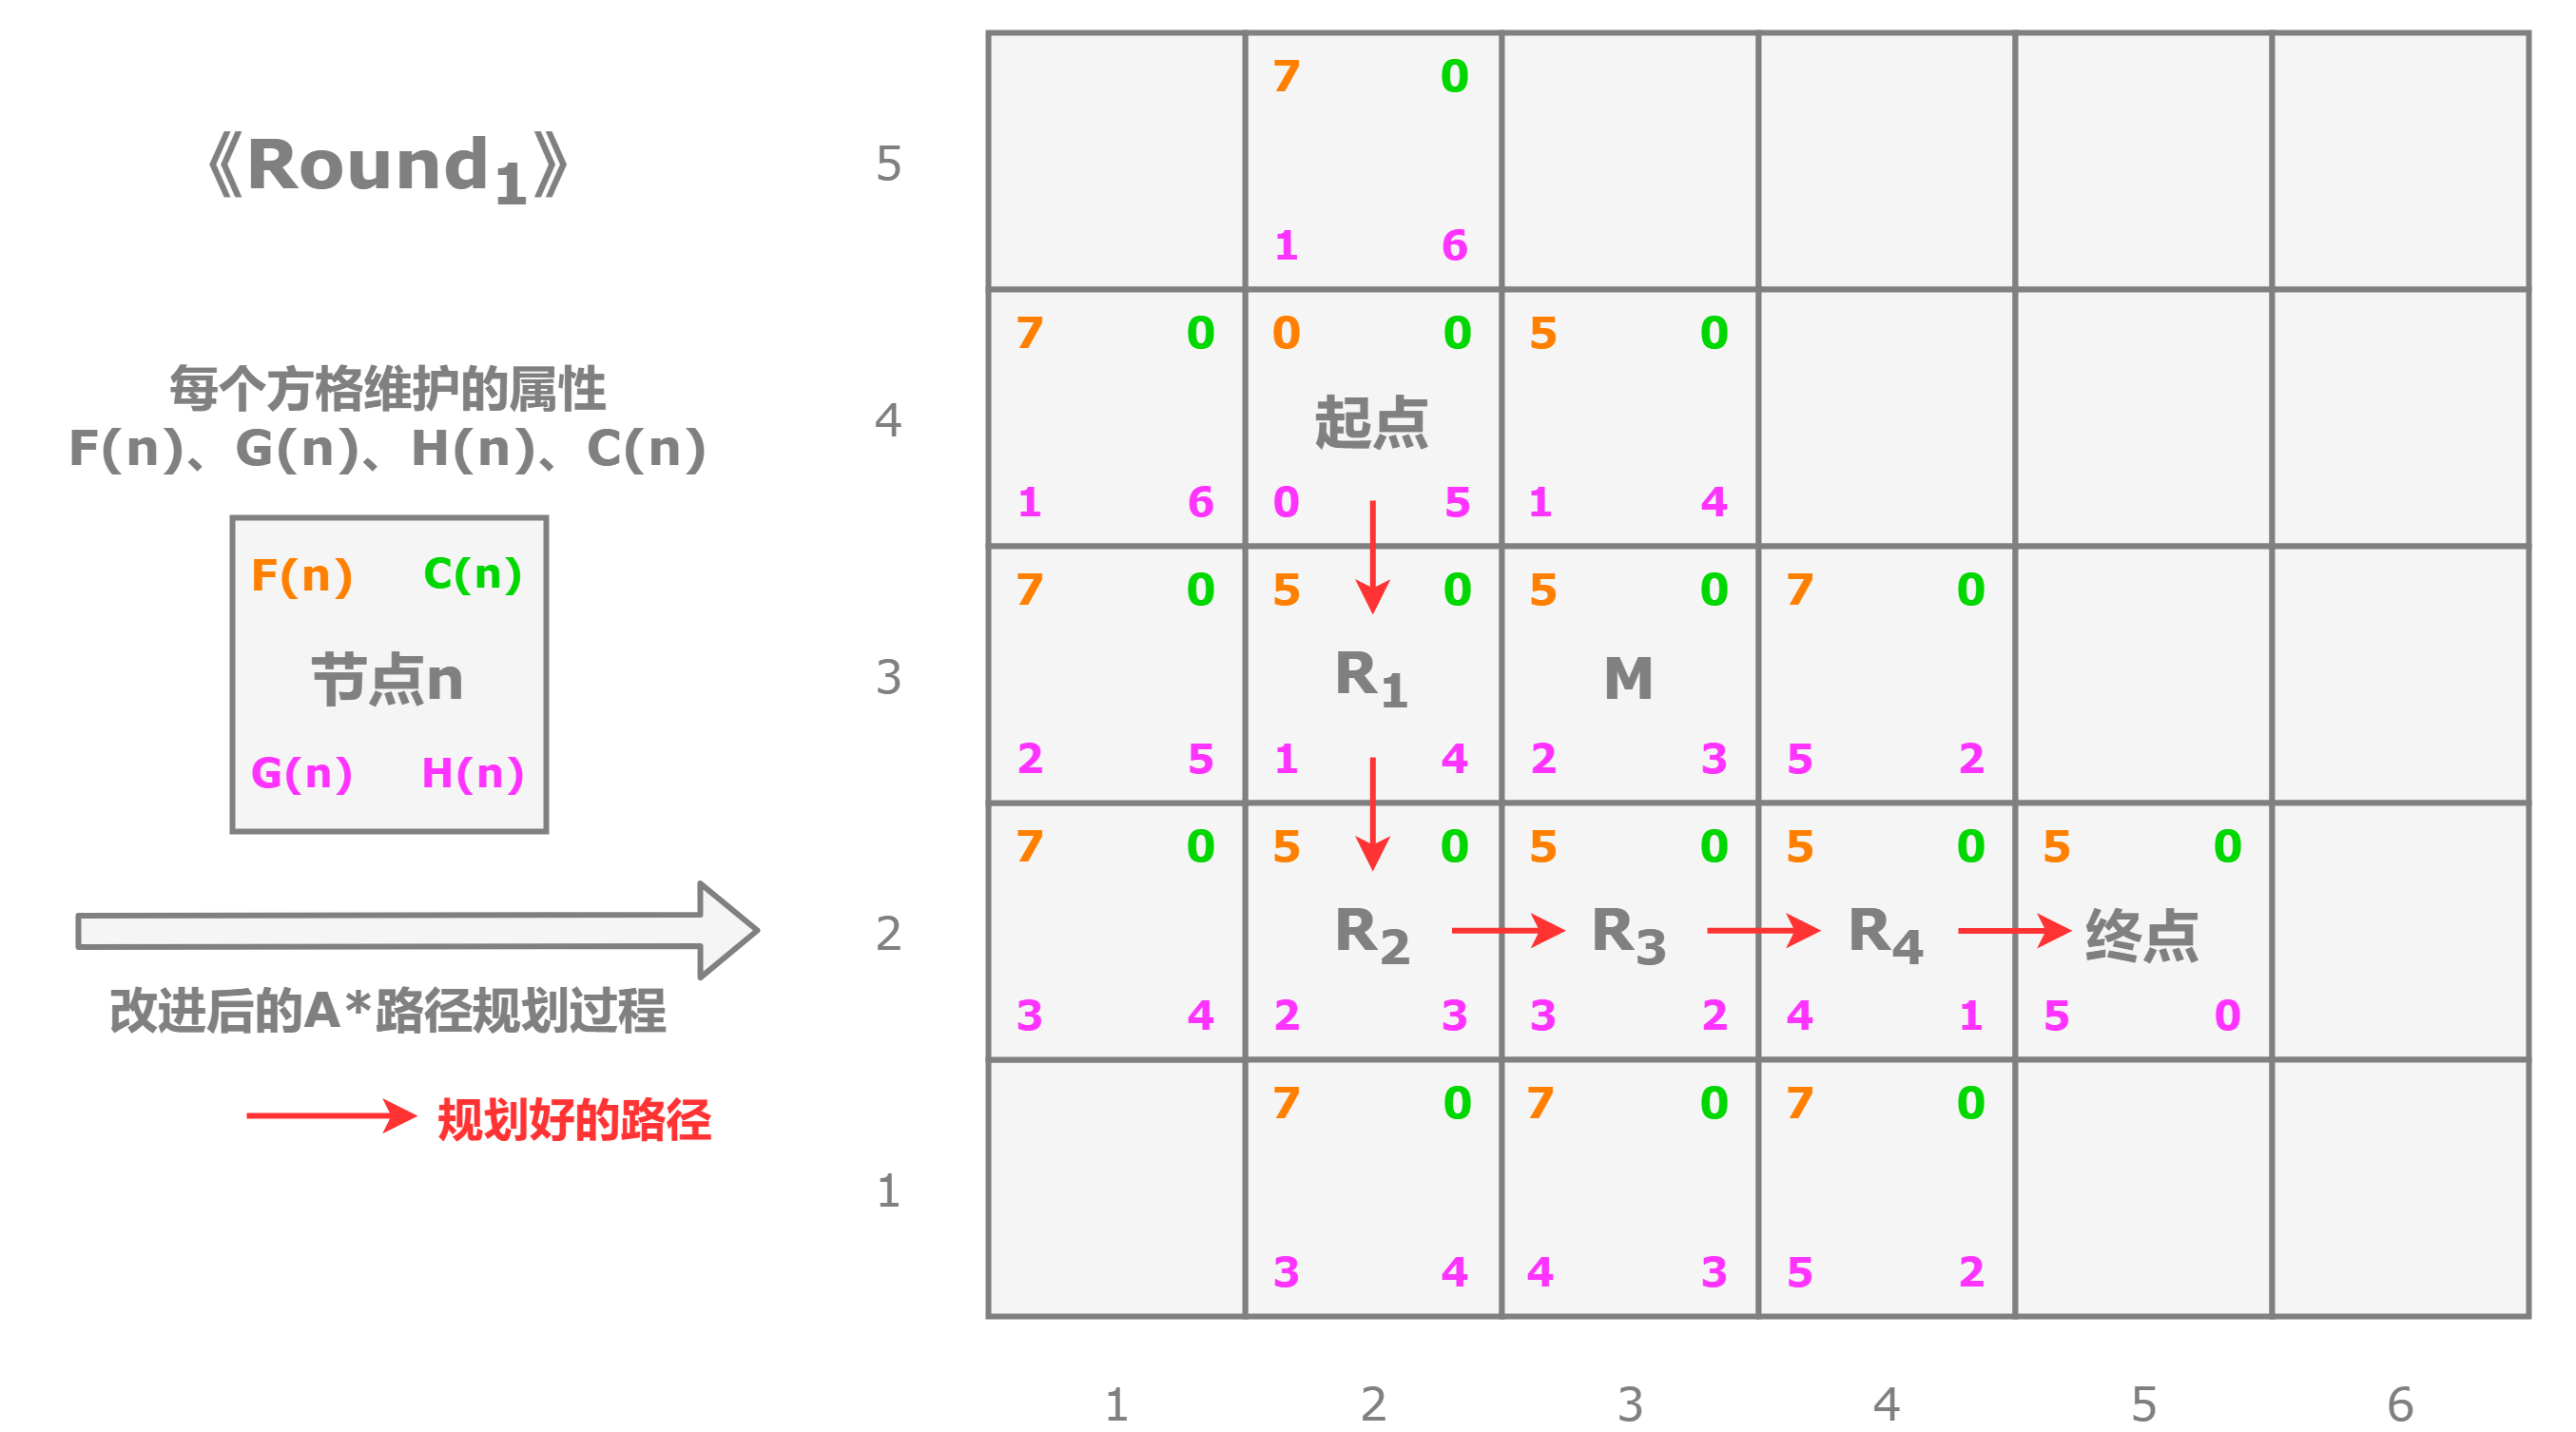
\includegraphics[width=0.75\textwidth]{undergraduate-thesis/images/Astar_newFnRound1.png}
  \caption{结合实时路况的改进A*算法($Round_1$)示例}
  \label{AstarnewFnR1} % label 用来在文中索引
\end{figure}

假设此系统一共运行2轮,在第1轮运行时,由于此前从未有车辆在该地图上行驶过,则第1轮运行时,所有道路的$V_{path}$都与道路的限速$V_{default}$一致,即此时相当于没有上一轮的实时路况,结合实时路况的改进A*算法规划出的路径与A*算法规划出的路径是一致的,如图\ref{AstarnewFnR1}中所示结果,规划出的路径为:起点 -> $R_1$ -> $R_2$ -> $R_3$ -> $R_4$ -> 终点。

由于第1轮车辆完成了一轮运行,此时已存储了$Round_1$的路况信息,则该路况信息将对$Round_2$中的路径规划产生影响。

\begin{figure}[ht]
  \centering
  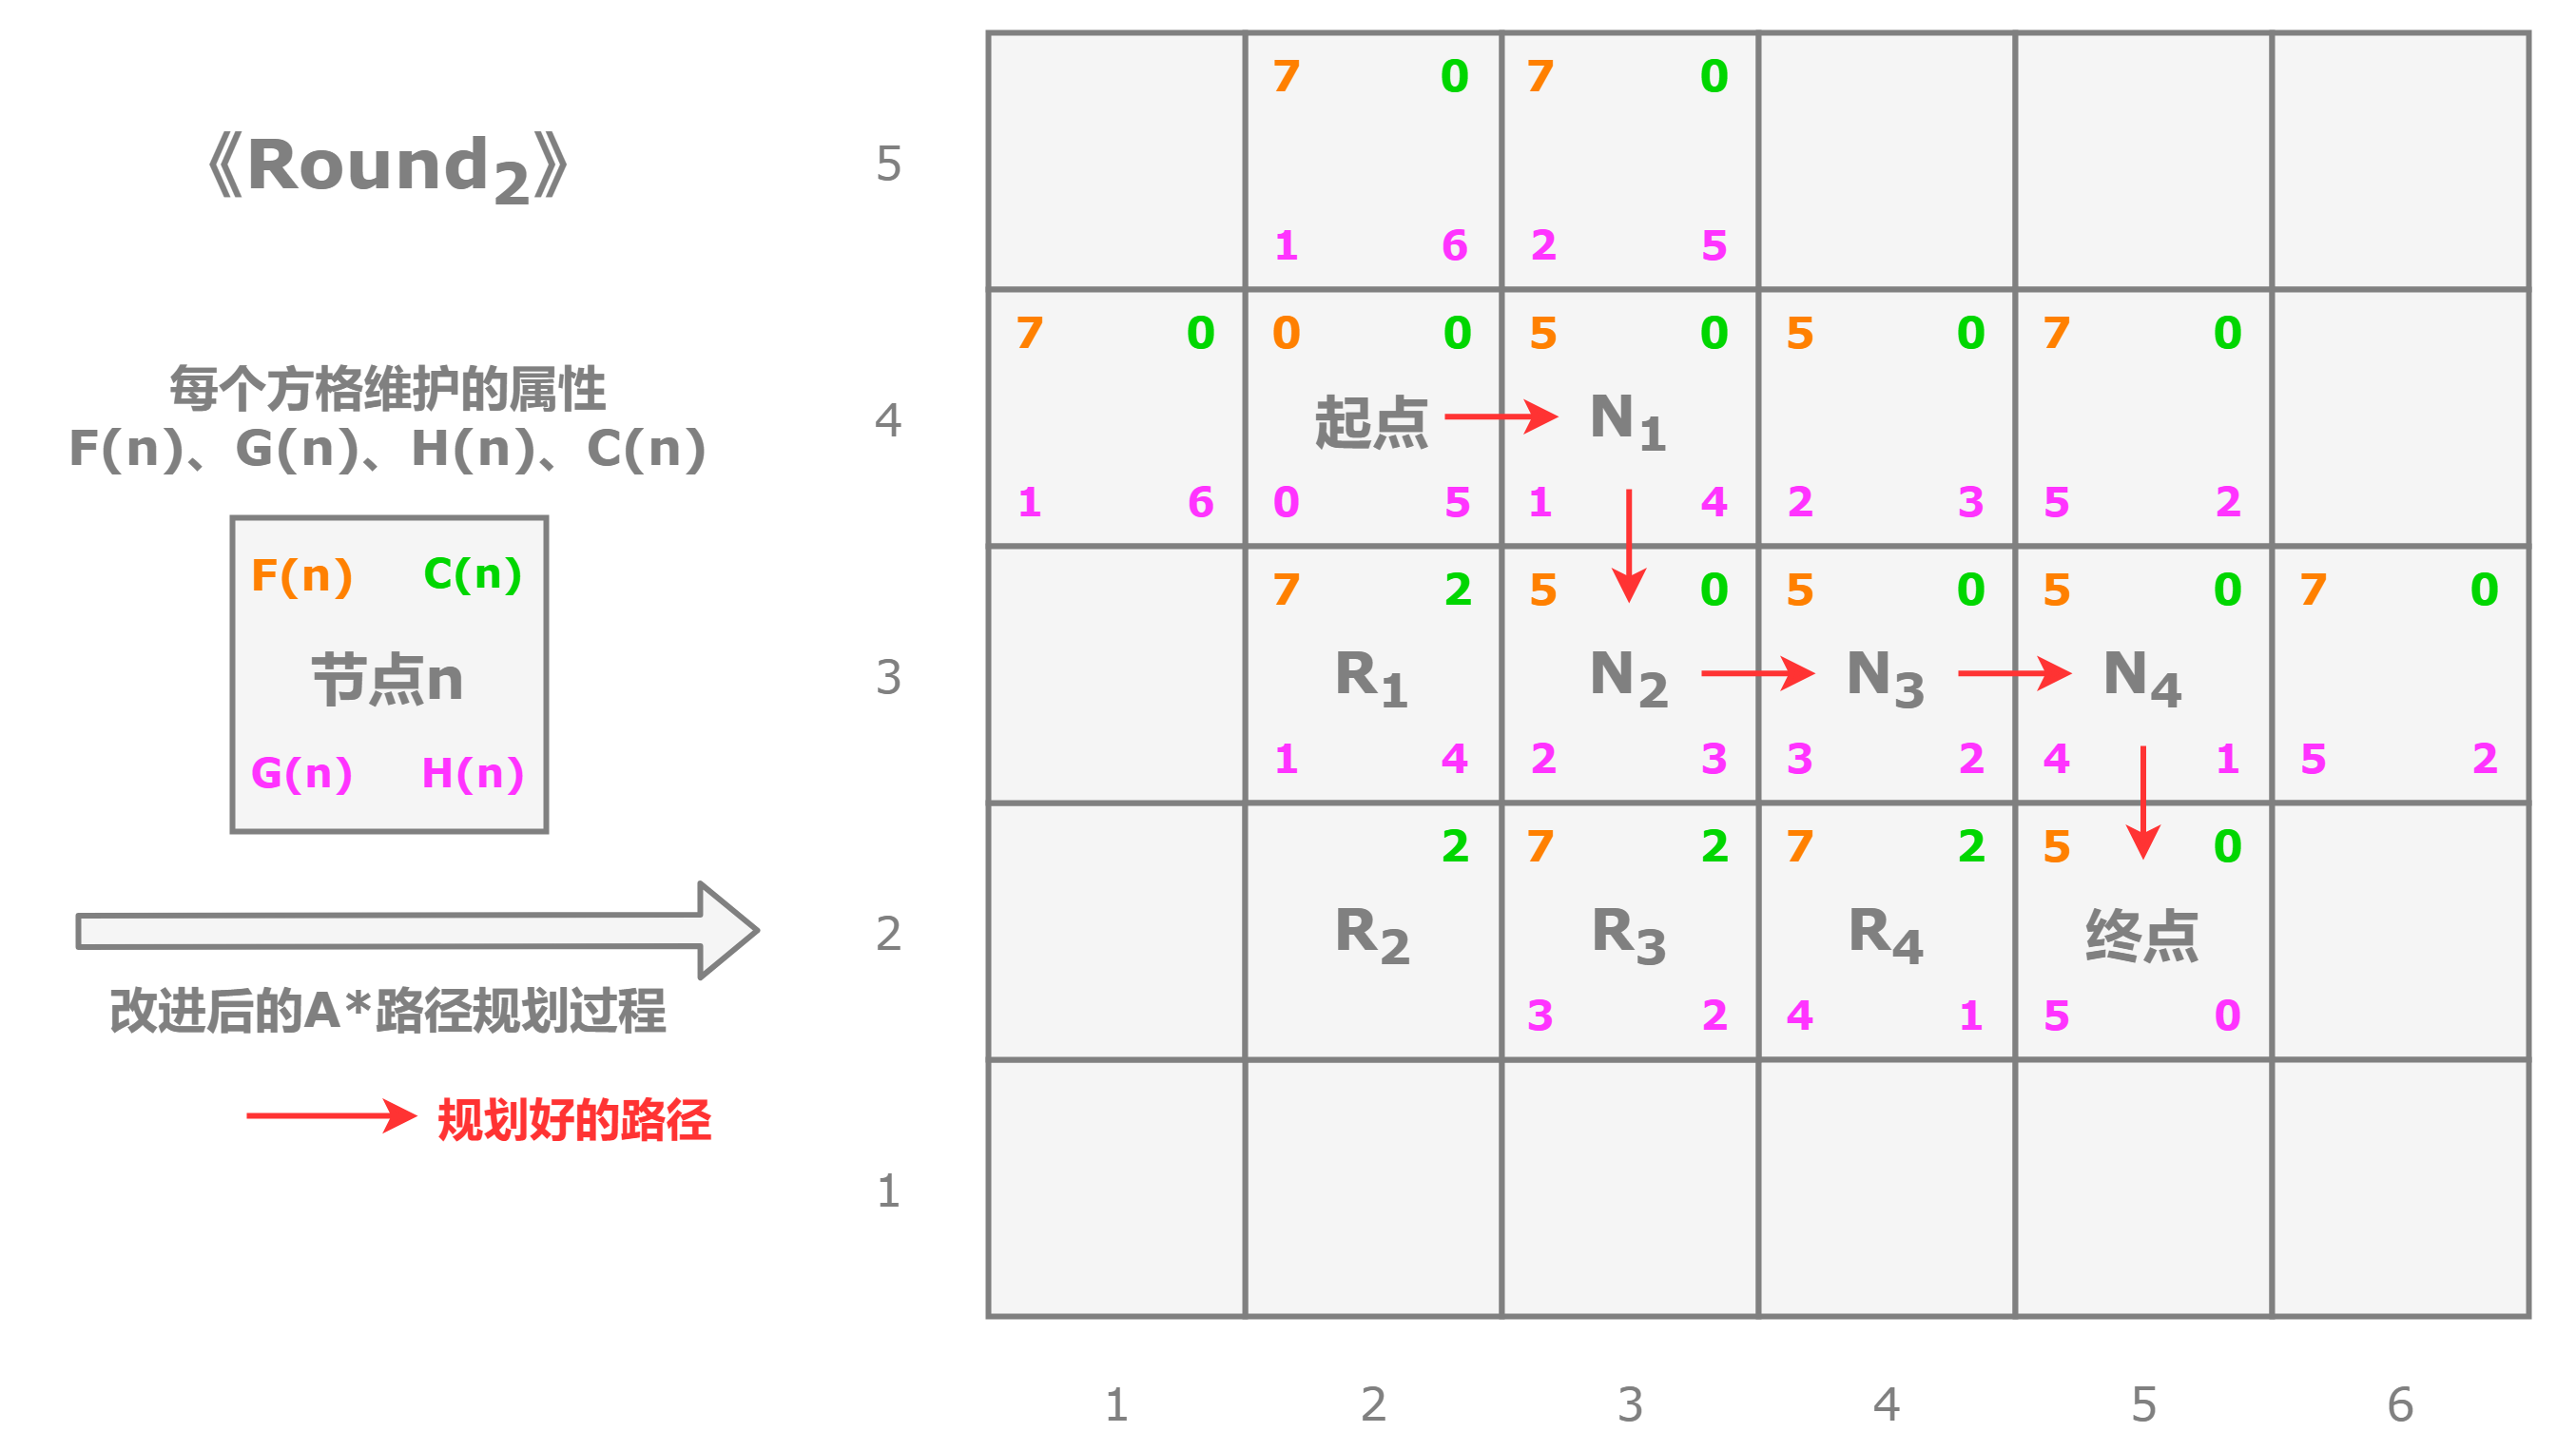
\includegraphics[width=0.75\textwidth]{undergraduate-thesis/images/Astar_newFnRound2.png}
  \caption{结合实时路况的改进A*算法($Round_2$)示例}
  \label{AstarnewFnR2} % label 用来在文中索引
\end{figure}

$Round_1$中规划好的路径,视作已经有车运行过了,为已走过的道路($R_1$、$R_2$、$R_3$、$R_4$)赋C(n)=2,则在$Round_2$中车辆再次从起点驶向终点时,路径规划的过程如图\ref{AstarnewFnR2}所示,结合实时路况的改进A*算法在$Round_2$中的运行过程为:

\begin{enumerate}
    \item 从起点到$N_1$点(第1轮):将起点位置加入Open表,然后从起点向外寻找。首先找到的是起点的上下左右四个邻居方格,将它们加入Open表里,将起点加入Close表。分别计算这四个邻居方格的总距离代价F,得出起点右侧邻居的F最小,则车辆向右侧移动,移至$N_1$点位,同时将$N_1$加入Close表中。
    \item 从$N_1$点到$N_2$点(第2轮):在$N_1$点位搜索邻居方格,发现起点作为$N_1$的左侧点位,实际上已经进入Close表中,因此,将$N_1$的上、右、下侧三个点加入Open表,作为邻居方格,并分别计算这三个邻居方格总距离代价F,得出$N_1$下侧和右侧邻居的F同时最小,按照假设,车辆向下侧移动至$N_2$点位,将同时将$N_2$加入Close表中。
    \item 从$N_2$点到$N_3$点(第3轮):在$N_2$点位搜索邻居方格。$N_2$点位的左、右、下侧三个方格作为邻居方格,但$R_1$格实际上已经在第1轮中计算过F,因此,此时重新计算$R_1$的总距离代价,所得代价较第1轮计算更高,因此不更新$R_1$在Open表中对应的F值。计算得到移动的下一个位置是$N_3$,将车辆移至$N_3$。
    \item 从$N_3$点到$N_4$点(第4轮):在$N_3$点位搜索邻居方格,将$N_3$的上、下、右侧三个方格作为邻居方格加入Open表中计算代价F。得出$N_3$上侧和右侧邻居的F同时最小,按照假设,车辆向右侧移动至$N_4$点位,将同时将$N_4$加入Close表中。
    \item 从$N_4$点到终点(第5轮):在$N_4$点搜索邻居方格,将$N_4$的上、下、右侧三个邻居列入本轮的总距离代价计算过程中,结果是移至终点的F最小,因此将终点加入Close表,车辆的当前位置移动为终点,则路径规划成功,算法运行结束。
\end{enumerate}

在此例中,经过$Round_1$与$Round_2$两轮运行后,A*算法在$Round_2$中寻得的路径为:起点 -> $N_1$ -> $N_2$ -> $N_3$ -> $N_4$ -> 终点。达到了路径规划基于实时路况而实时更新的结果,说明此算法是正确且可行的。

\section{结合实时路况的改进A*算法在调度系统中的实现}
\label{section_useNewAstarinTaxiSystem}
% 更新——————————————
Solidity语言是一种面向智能合约的、图灵完备的高级编程语言,它由以太坊提供,在以太坊虚拟机(EVM)上运行。Solidity是面向对象的语言,它具有静态的特性,支持继承、类库、用户自定义类型等特性。Solidity是目前较常应用于以太坊的语言。Remix-ide是一款基于浏览器的Solidity编译器,它可以在线使用。本文使用Solidity语言完成智能合约的开发,使用Remix-ide完成对智能合约的编译。

\begin{figure}[ht]
  \centering
  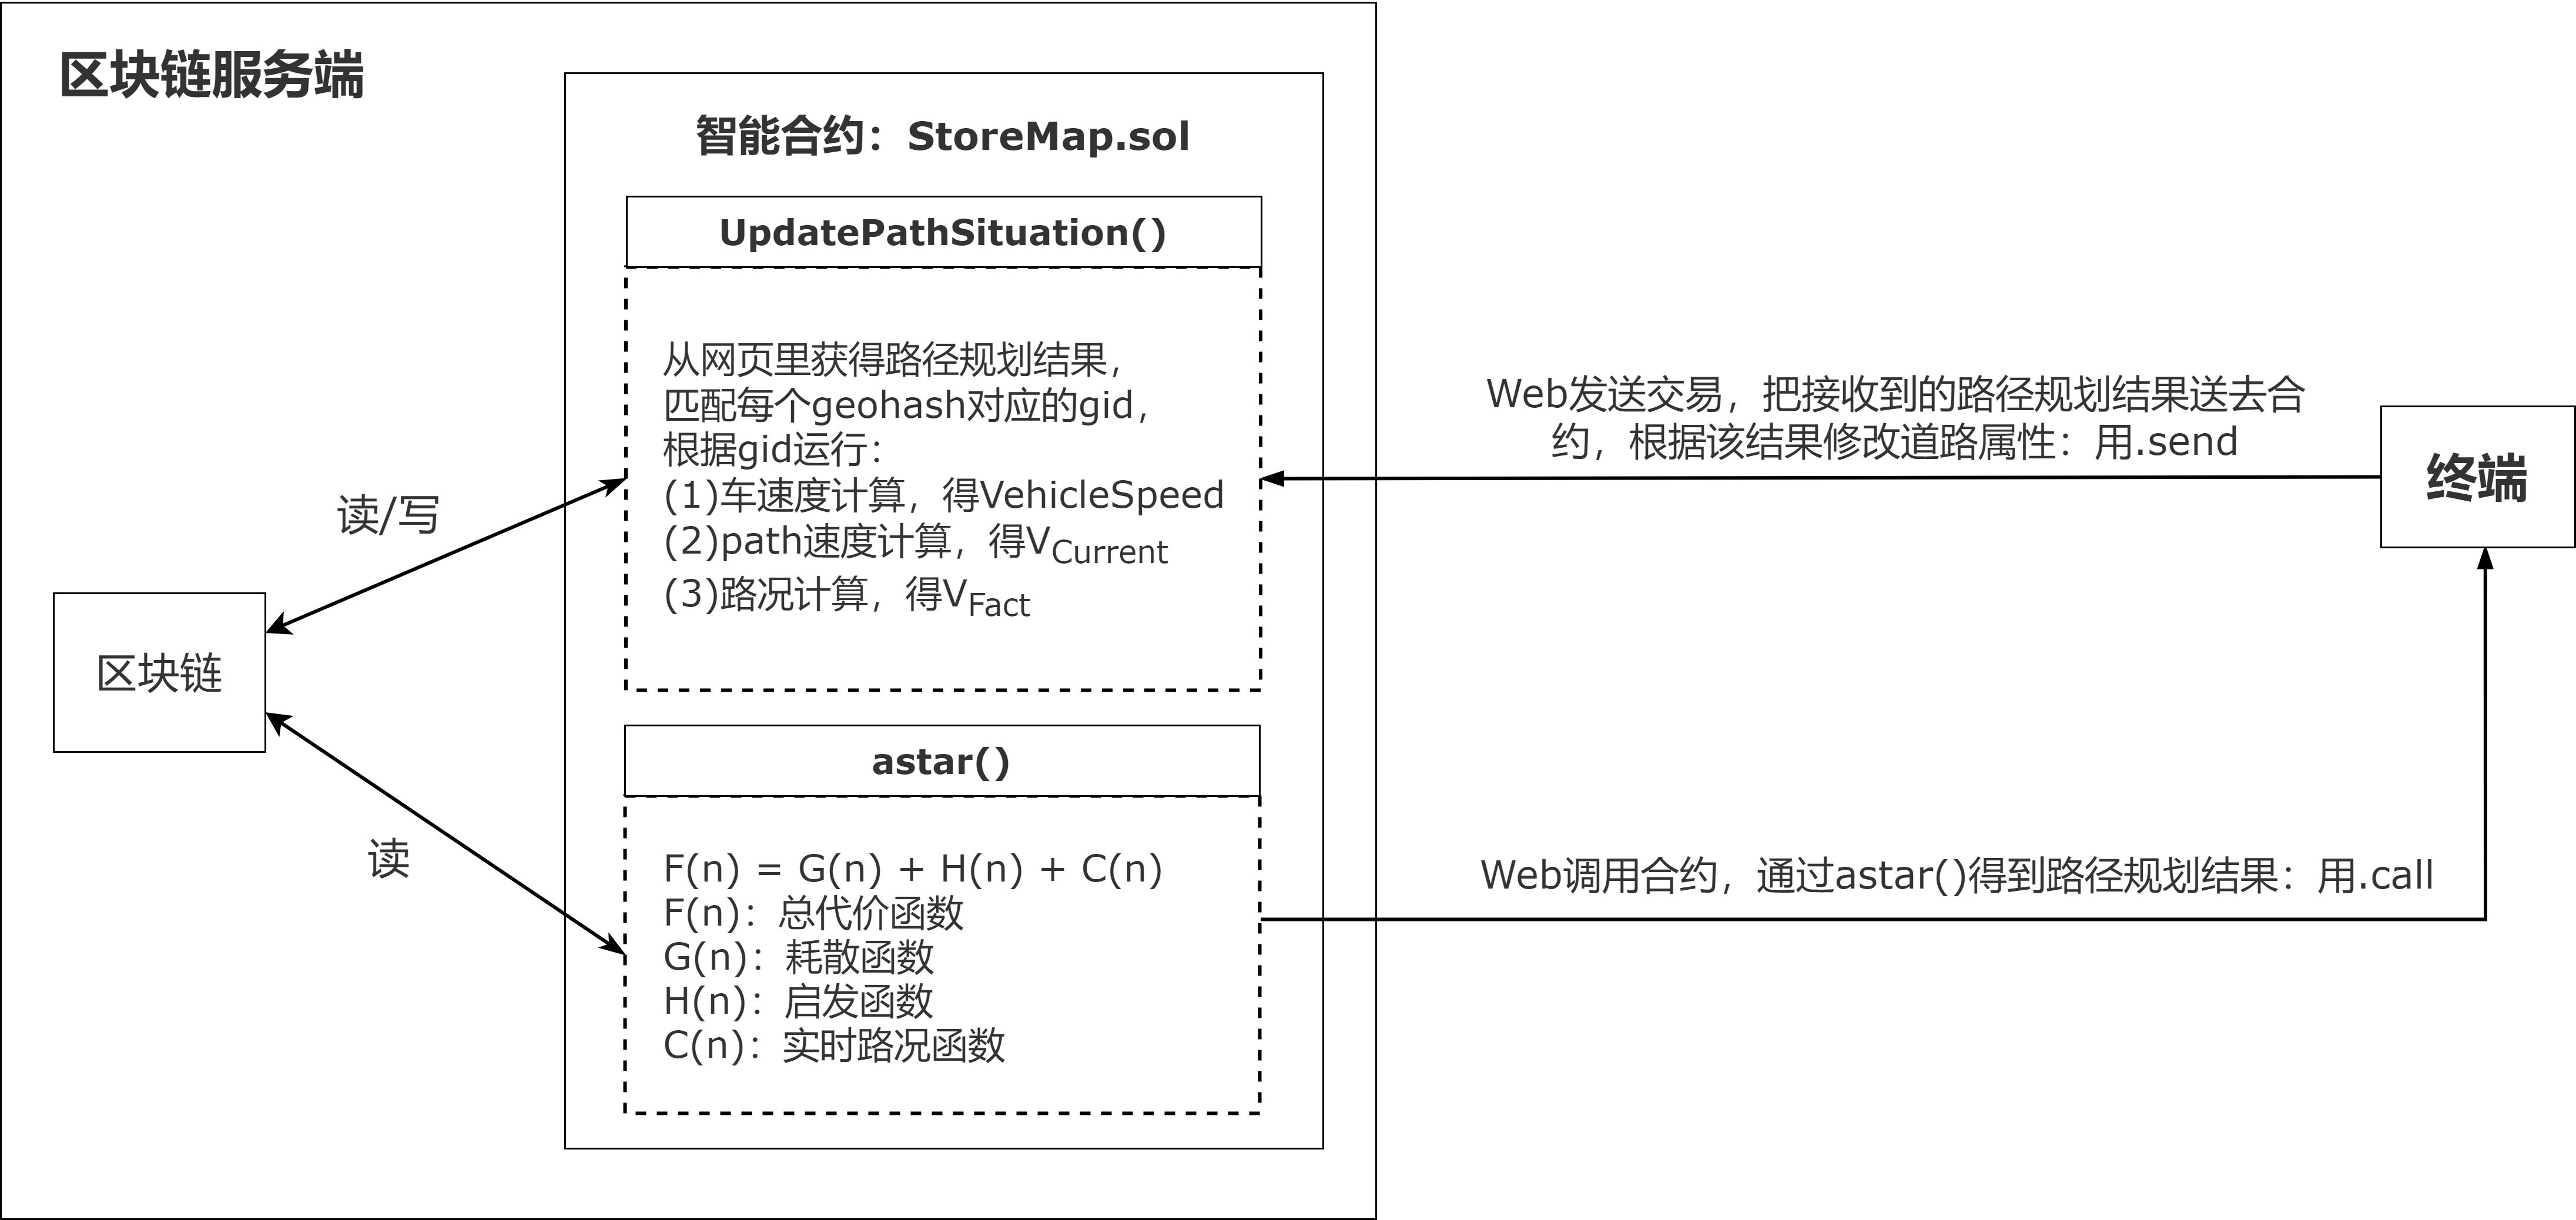
\includegraphics[width=0.8\textwidth]{undergraduate-thesis/images/AlgorithmInteractive.png}
  \caption{实现思路示意图}
  \label{algorithm-interactive} % label 用来在文中索引
\end{figure}

在已有的出租车调度系统中,主要的实现思路如图\ref{algorithm-interactive}。整个系统分为智能合约、区块链、网页端三大部分。智能合约部署在区块链上,由网页端通过调用智能合约内函数的方式与区块链交互。具体到本算法中,先打开树状区块链,在其上部署智能合约,并上传地图,最后打开python脚本用自动化工具selenium自动控制Web网页行为,运行系统。
% 设置三线表
\begin{table}[ht]
    \linespread{1.5}
    \zihao{5}
    \centering
    \caption{函数调用方法区别}
    \label{callandsend}
    \begin{tabular}{cc}
    \toprule
    .call & .send\\
    \hline
    不修改链上数据 & 修改链上数据 \\
    函数可以返回数据 & 函数不返回数据 \\
    函数立刻执行 & 函数花费一段时间执行完毕 \\
    免费 & 花费gas \\
    \bottomrule
    \end{tabular}
\end{table}
% 结束设置三线表

智能合约中,UpdatePathSituation()用于实时路况的计算和更新,它对链上存储的数据进行读和写操作;astar()用于运行改进的A*算法规划路径,它只需要对链上数据进行读取。因此这两个函数在调用时,参考表\ref{callandsend},前者用call调用,后者用send调用。

Web网页通过调用astar()来完成基于实时路况的路径规划,在获取到改进A*算法调度出的路径之后,将此路径规划结果打包为交易的方式,以输入参数的形式提交给UpdatePathSituation(),通过智能合约修改区块链上与实时路况相关的道路属性数据,实现实时路况的更新。在系统的下一轮运行时,Web网页再次调用astar(),就将根据区块链上新的道路属性数据计算道路的总距离成本,实现路径规划,从而进行动态路径规划过程。

在已有的出租车调度系统中一共需要部署3个合约,这三个合约分别被命名为StoreMap.sol、StoreTraffic.sol、Credit.sol。StoreMap.sol的功能是完成地图的存储、前端的匹配、用A*算法实现路径规划;StoreTraffic.sol的功能是进行车辆与乘客的系列操作(包括初始化车辆与乘客的位置、设置车辆与乘客的起点和终点、修改乘客与车辆的状态等)、乘客确认上车、乘客支付路费、存储和获取A*算法计算所得的路径;Credit.sol的功能是完成车辆信誉值的计算。

\begin{figure}[ht]
  \centering
  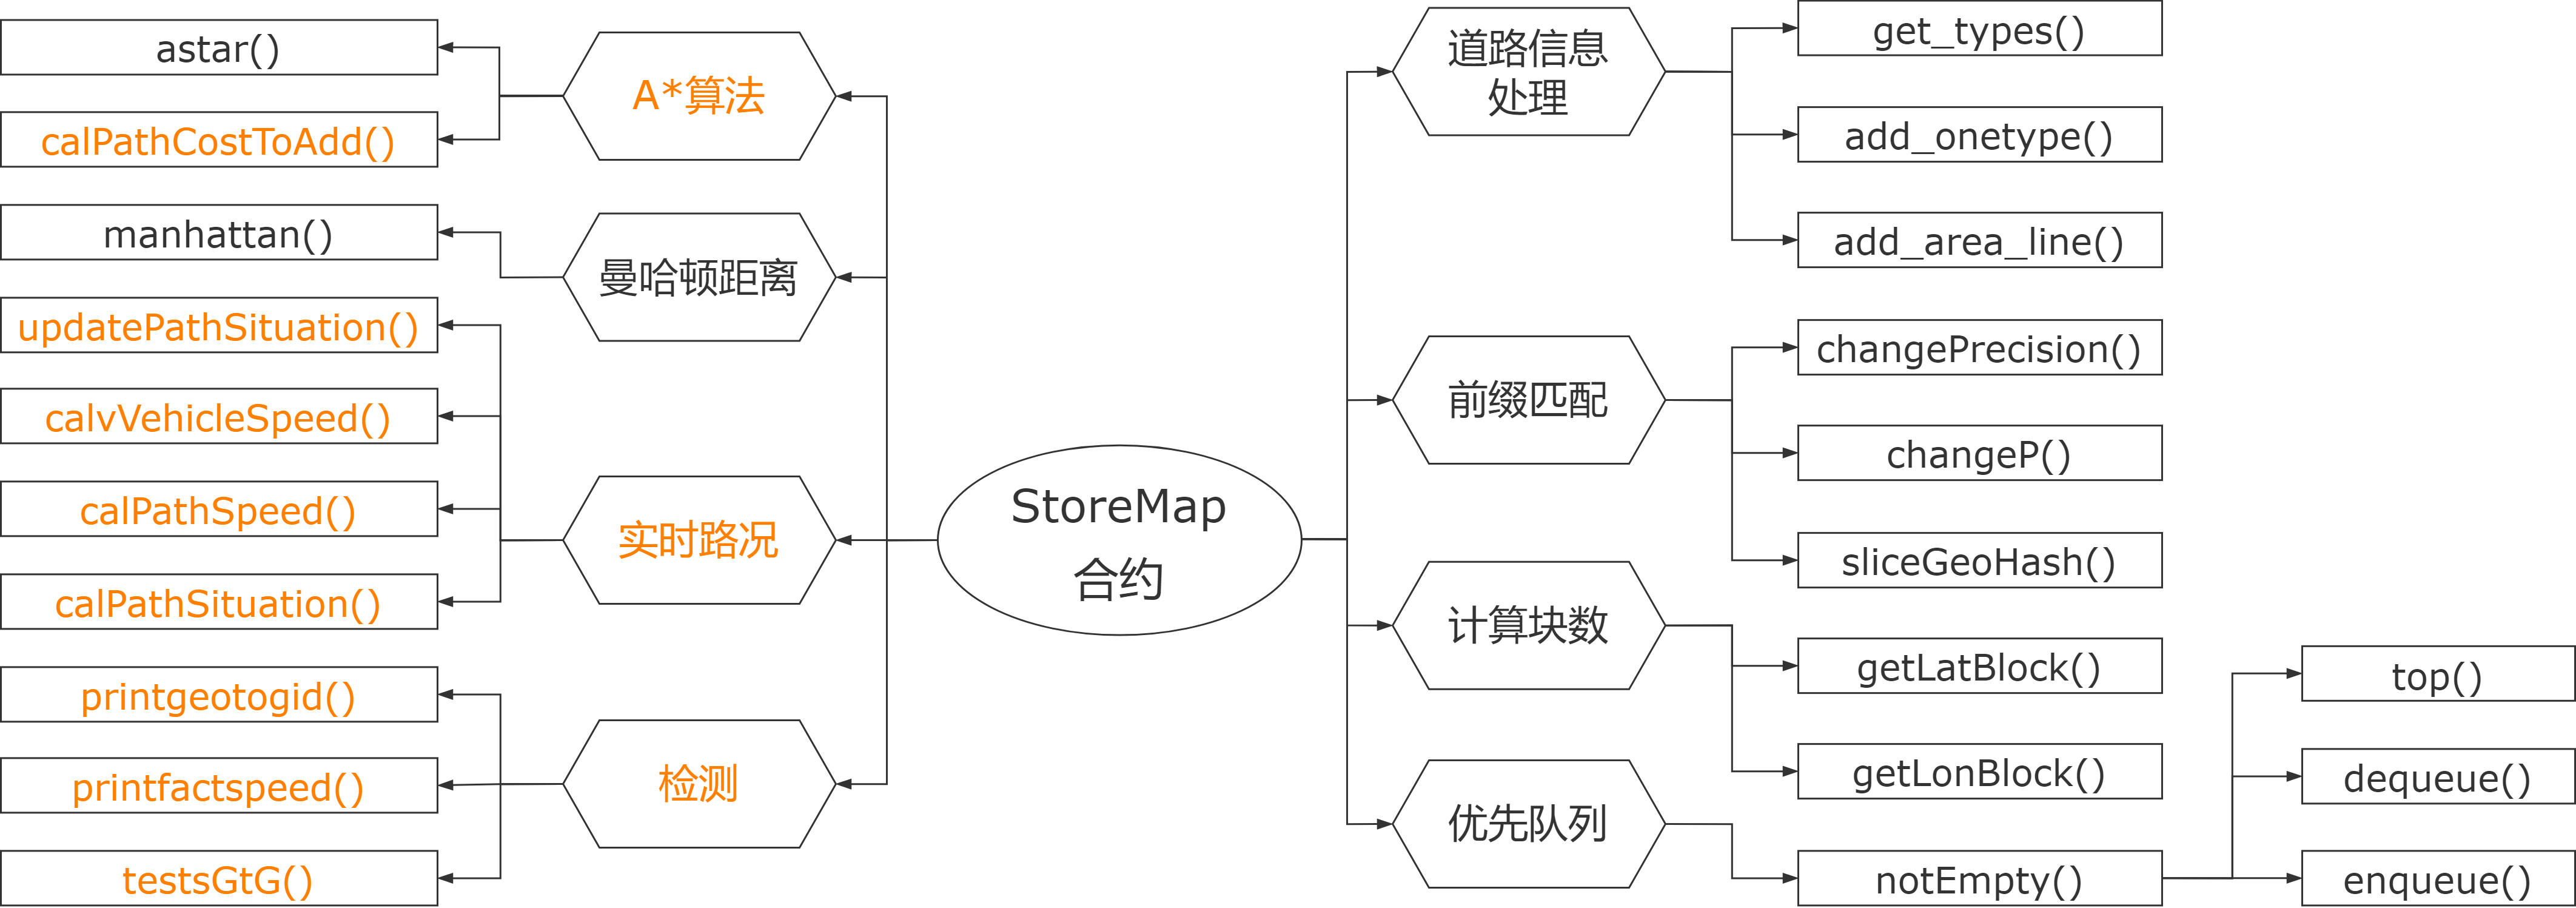
\includegraphics[width=1\textwidth]{undergraduate-thesis/images/StoreMapContract.png}
  \caption{StoreMap.sol架构示意图}
  \label{SMContract} % label 用来在文中索引
\end{figure}

本文将出租车调度系统中的寻路算法更新为结合实时路况的改进A*算法,主要做的修改是在智能合约StoreMap.sol中。图\ref{SMContract}是合约StoreMap.sol的架构示意图。黑色的函数对应的是合约中原有的函数,本文在其基础上,补充了计算实时路况、检测这两个模块;接下来,本文补充了calPathCostToAdd()函数,其归类在A*算法模块下,在同模块的astar()函数中调用,对总距离代价F的计算公式也做了对应修改;本文还补充了将Geohash值映射为路段gid值的mapping结构,在使用add\_onetype()存储路径时对其进行写操作,以方便用Geohash值对路段进行查询的读操作。

由于本文工作未对StoreTraffic.sol、Credit.sol进行修改,因此本文未对这两个合约的架构示意图进行分析展示。

本文所依赖的出租车调度系统有两种运行模式,一种是借助前端进行运行,在浏览器网页中,可以可视化看到向区块链里上传好的地图、A*算法规划完毕的路径、乘客和车辆不同时间段的状态、系统内部的某些变量等系统运行细节;另一种是借助控制台直接运行测试脚本,在控制台里,可以输出各环节乘客和车辆的不同状态、以Geohash编码的形式输出A*算法规划完毕的路径、输出系统内部的某些变量值,但无法可视化看到规划好的路径,可视化看到区块链中存储的地图。

但无论是借助前端运行还是借助控制台运行,本出租车调度系统与区块链中部署的智能合约的交互过程都是通过调用合约内容、向区块链提交交易完成的。两种运行方式的不同之处仅仅在于是否调用前端做出类似打车软件一样的可视化效果。因此,本文接下来将以借助前端运行的过程为例,阐明结合实时路况的改进A*算法应该如何在出租车调度系统中完成调用过程。
% 图得再改,改成能看清字的,只放函数名称得了
\begin{figure}[ht]
  \centering
  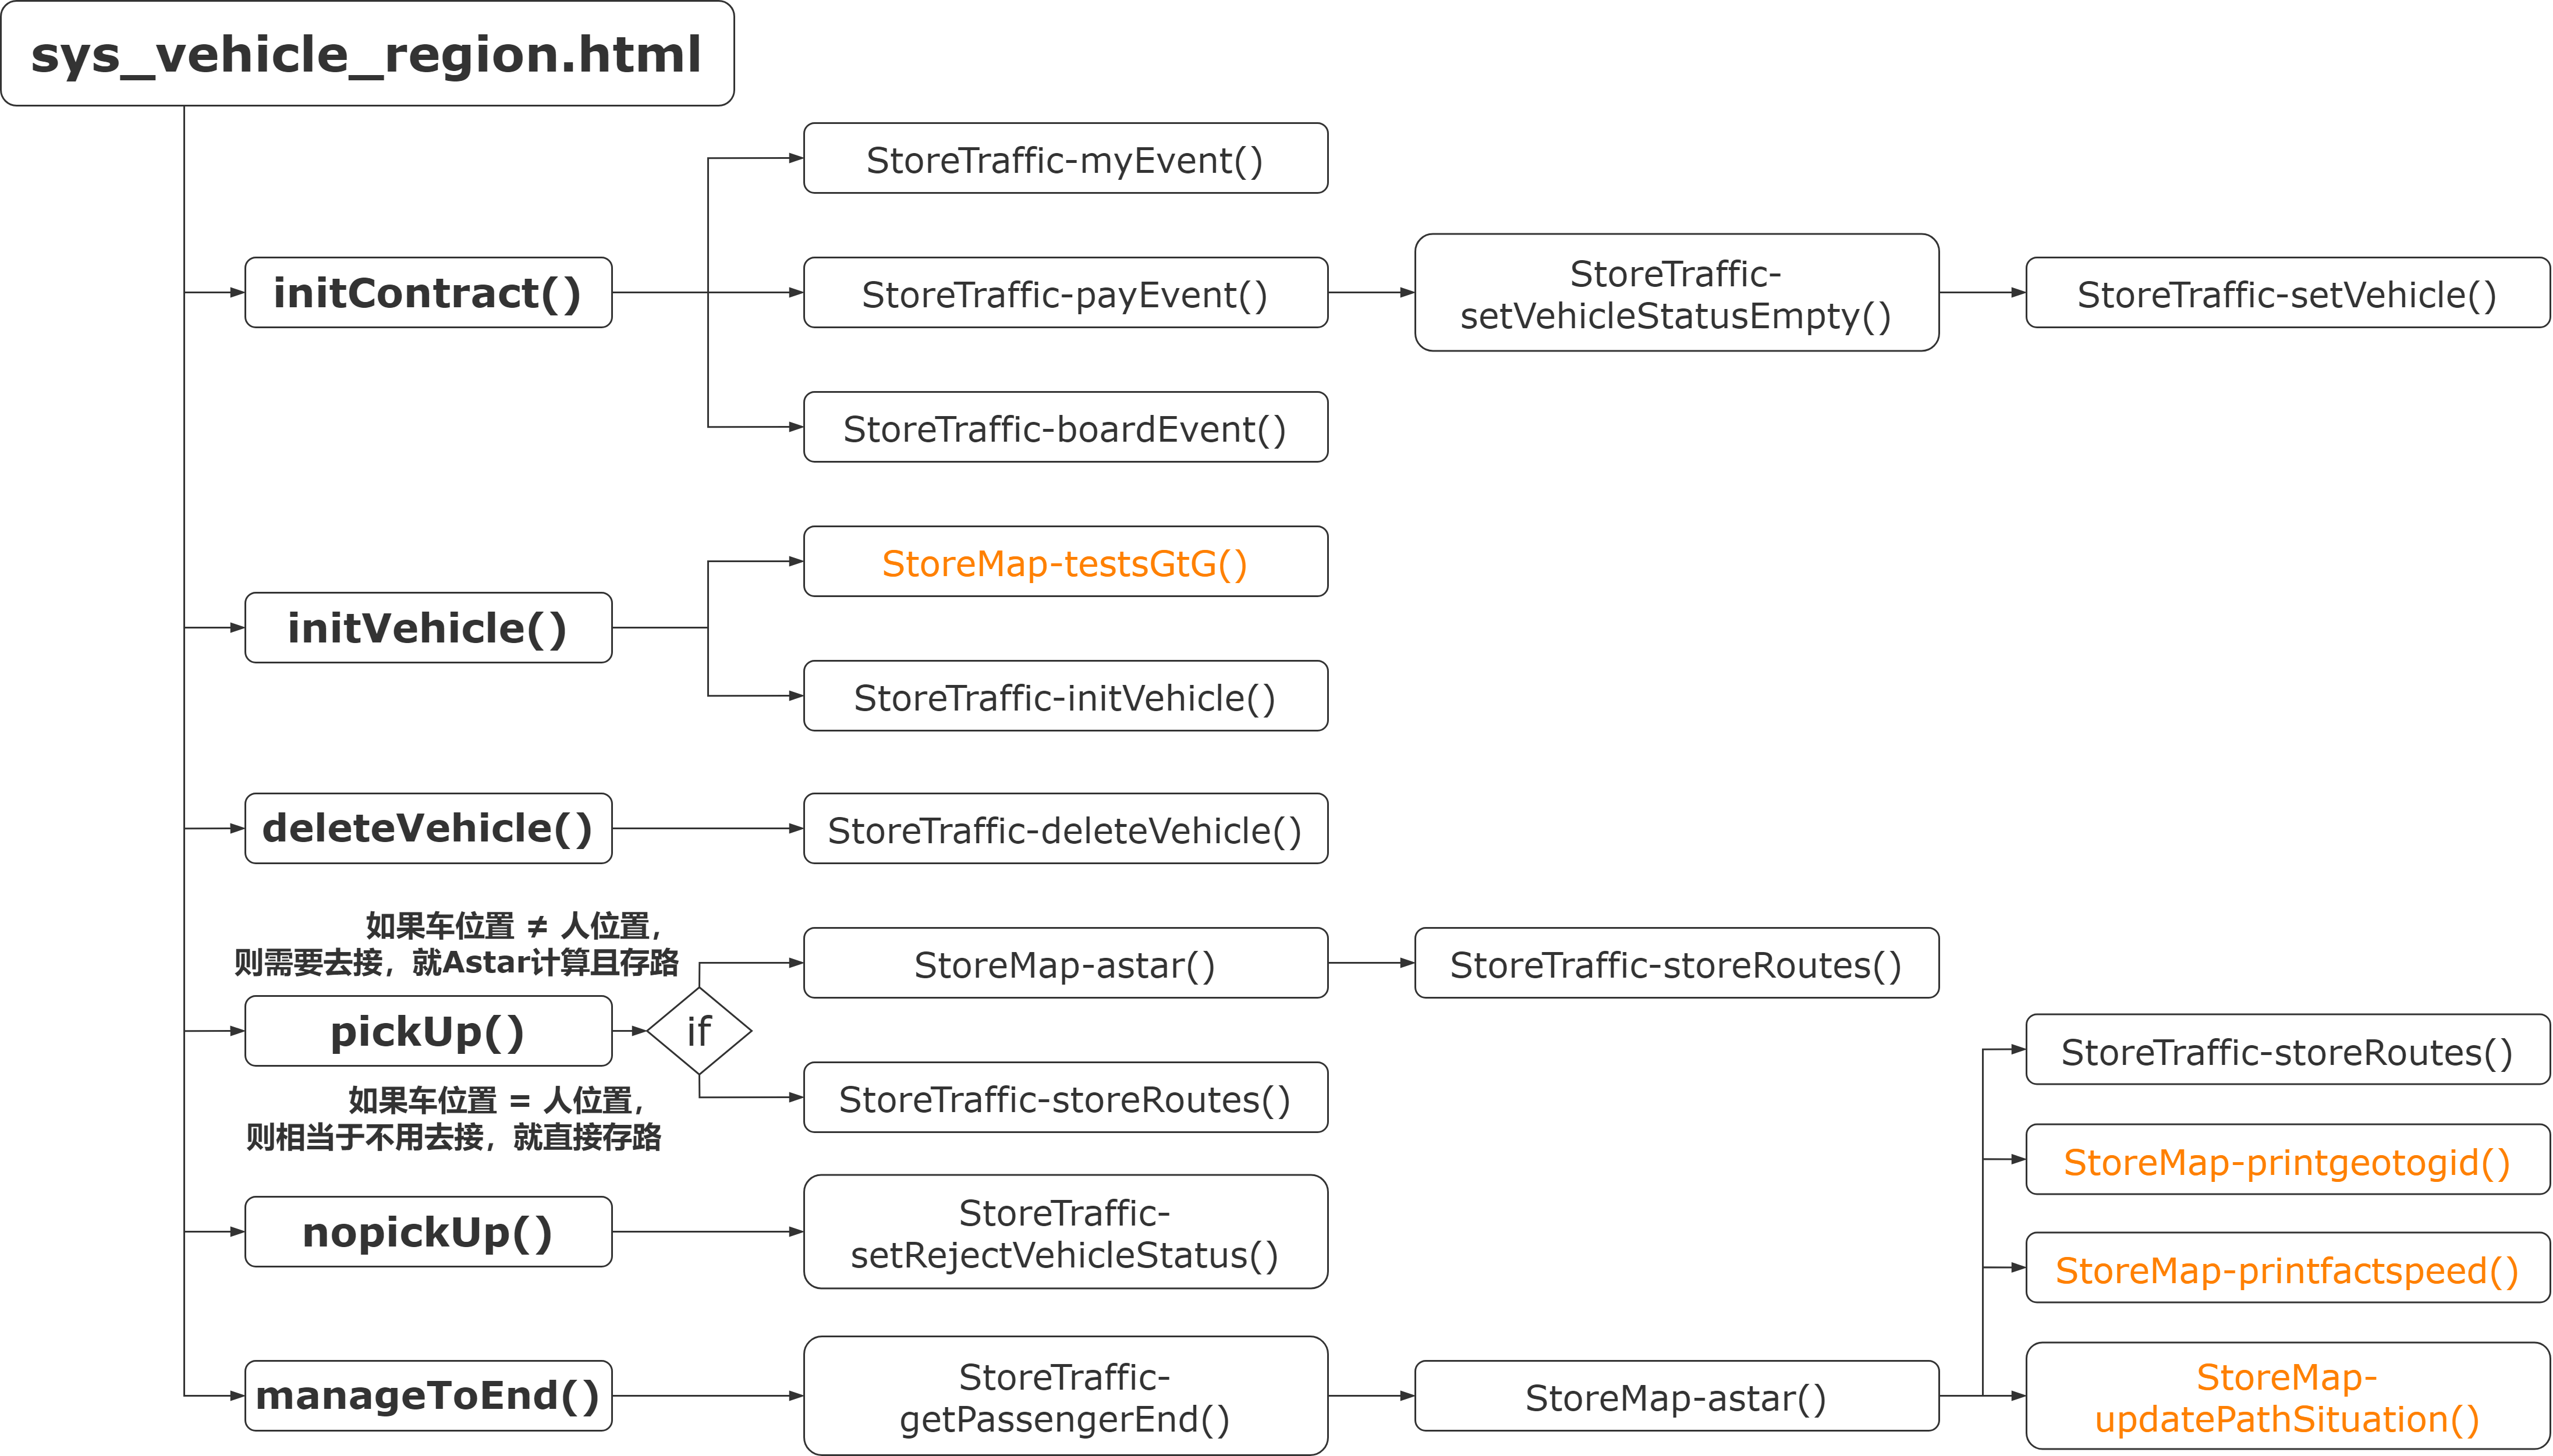
\includegraphics[width=1\textwidth]{undergraduate-thesis/images/callContracts_vehicle.png}
  \caption{车辆端Vehicle调用智能合约的逻辑示意图}
  \label{callContractsV} % label 用来在文中索引
\end{figure}

图\ref{callContractsV}展示了在出租车调度系统运行时,车辆端Vehicle所对应的前端网页调用智能合约的逻辑。它一共拥有6个主要的函数。黑色的合约函数是本系统中已有的,橙色的合约函数是本文为实现动态的路径规划而添加的调用过程。

1.initContract():初始化合约、监听前端事件发生。这个函数监听前端发生的乘客发起乘车请求、车辆接到乘客、乘客支付成功等事件,并根据事件种类调用不同函数。当MyEvent事件触发时,说明乘客发出订单,此时进行pickUp()过程,车辆由车辆位置前往乘客起点,在此期间需要使用合约中astar()函数进行一次动态路径规划;当boardEvent事件触发时,说明车辆已经接到乘客,此时进行manageToEnd()过程,车辆由乘客起点前往乘客终点,在此期间需要使用合约中astar()进行一次动态路径规划、使用合约中updatePathSituation()进行一次实时路况更新。

2.initVehicle():初始化车辆信息。它调用合约中initVehicle()来完成:上传车辆位置、初始化车辆状态的作用。本文在此函数中添加了对合约中testsGtG()函数的调用,目的是为了测试地图上传时,合约是否能正常存储Geohash到gid的映射关系。

3.deleteVehicle():删除车辆信息。系统每个轮次结束运行后,乘客到达终点并完成支付,车辆被认为完成此次运行,因此删除本轮次已经完成运行的车辆信息。

4.pickUp():接乘客过程模拟。该函数出现在系统运行的第一个重要阶段,此时乘客和车辆都已完成初始化,乘客发出了打车请求,并且通过区块链完成对车辆的呼叫,车辆接单,此时通过pickUp()来完成从车辆的初始位置运行到乘客的起点,实现接到乘客的效果。该过程主要调用合约内astar()函数,astar()函数规划一条以车辆位置为起点、以乘客起点为终点的道路。

5.nopickUp():车辆拒接乘客。该函数调用合约中setRejectVehicleStatus()函数来完成拒接效果。

6.manageToEnd():送乘客过程模拟。该函数出现在系统运行的第二个重要阶段,此时车辆已接到乘客。此过程调用合约中astar()函数,通过区块链完成动态路径规划,给出从乘客起点到乘客终点的行驶路径,从而完成乘客此次订单,并调用合约中updatePathSituation()函数完成对当前轮次运行过程的实时路况的计算,并将该计算结果存进区块链。

由于基于实时路况的改进A*算法在出租车调度系统里只在车辆Vehicle端被调用,在实现改进的A*算法的过程中不需要对乘客Passenger端的合约调用逻辑进行修改,因此本文未对乘客Passenger端的合约调用逻辑进行分析展示。

\section{本章小结}

首先,本章介绍了基于区块链的出租车调度系统的整体结构。

接着,本章从传统A*算法的公式引入,介绍了传统A*算法所依赖的总距离代价函数F(n)的计算方式。F(n)由耗散函数G(n)和启发函数H(n)构成,G(n)的计算过程和结果一般固定,但启发函数H(n)有不同的计算方式,且选取不同方式得出的计算结果会存在差异。结合本系统向区块链上传的地图特性与出租车调度系统是基于城市横平竖直的街道运行的特点,本文最终选取曼哈顿距离作为A*算法的启发函数H(n)进行计算。接下来,本章结合传统A*算法的流程图和简单的例子,对传统A*算法规划路径整体过程进行了阐述。随后,本章根据A*算法的特性给出了设计结合实时路况的改进A*算法的必要性。

本章在第\ref{A*New}节从计算实时路况、改进A*算法总距离代价计算公式的两个环节阐明了改进A*算法的思路与过程,并强调了在计算实时路况时要注意影响因子的选取结果,接下来借助第\ref{A*Reason}节中的情景,描述了结合实时路况的改进A*算法的路径规划过程和预期效果。

最后,通过分析智能合约的实现逻辑、出租车调度系统与区块链交互时调用智能合约的逻辑,本章在第\ref{section_useNewAstarinTaxiSystem}节中给出了改进A*算法在出租车调度系统中的具体实现方法,并对出租车调度系统调用A*算法的整体逻辑进行了介绍。